% ============================================================================
% LAFC-Evict manuscript -- Performance Evaluation (Elsevier) template.
%
% MECHANICAL TEMPLATE MIGRATION NOTICE
% -------------------------------------------------------------------------
% This file is a mechanical reformatting of the canonical SIGMOD manuscript at
% paper/sigmod2027/latex/main.tex (ACM `acmart` class) into the Elsevier
% `elsarticle` class for submission to Performance Evaluation. No scientific
% content, results, numbers, or claims were changed. See
% paper/performance_evaluation/TEMPLATE_MIGRATION_REPORT.md for the full
% audit of what changed and why.
%
% Elsevier guidance consulted 2026-09-13 (see migration report for links):
%   - ScienceDirect "Guide for authors" listing for Performance Evaluation
%     (elsarticle.cls, elsarticle-num citation style, Highlights mandatory)
%   - Elsevier "LaTeX instructions for authors" (elsarticle.cls current)
%   - Elsevier CRediT author statement policy
%   - Elsevier data statement / declaration-of-interest guidance
%   - Elsevier generative-AI-in-writing disclosure policy (updated 2026-06)
% ============================================================================
\documentclass[preprint,12pt]{elsarticle}

% Declares the target journal name in the running head of the preprint style.
\journal{Performance Evaluation}

% ---- Packages inherited unchanged from the SIGMOD manuscript ----
\usepackage{booktabs}
\usepackage{multirow}
\usepackage{enumitem}
\usepackage{array}
\usepackage{tabularx}
\usepackage{hyperref}
\usepackage{amsmath}
\usepackage{graphicx}

\newcommand{\lafc}{LAFC-Evict}
\newcolumntype{L}{>{\raggedright\arraybackslash}X}
\newcolumntype{P}[1]{>{\raggedright\arraybackslash}p{#1}}

\begin{document}

\begin{frontmatter}

% TEMPLATE NOTE: the SIGMOD source title carried a
% "\texorpdfstring{[Experiments \& Analysis]}{...}" suffix, which is a
% SIGMOD/VLDB "Experiments and Analysis" track label. That label is specific
% to the SIGMOD submission track and is not applicable to a Performance
% Evaluation journal submission, so it is dropped here as a venue-specific
% formatting artifact, not a scientific content change.
\title{\lafc: A Large-Scale Counterfactual Benchmark for Learned Cache Eviction}

% TEMPLATE NOTE: the SIGMOD manuscript listed "Anonymous Authors" for
% double-blind review. Performance Evaluation review is not double-blind at
% the author-facing template level, so real author/affiliation metadata is
% required. No author metadata was present in the SIGMOD manuscript itself;
% the identity below is taken from the repository's own CITATION.cff
% (repo root), which lists a single author. Please confirm this is complete
% and correct (co-authors, ORCID, grant/affiliation numbers) before
% submission.
\author[njit]{Soroush Vahidi\corref{cor1}}
\ead{sv96@njit.edu}
\cortext[cor1]{Corresponding author.}

\affiliation[njit]{organization={New Jersey Institute of Technology},
            city={Newark},
            state={NJ},
            country={USA}}

\begin{abstract}
\begin{sloppypar}
Judging a cache-eviction decision requires knowing what would have
happened under each candidate the system could have evicted instead --
information a single trace replay never reveals, since only one candidate
is actually evicted. This complicates comparisons across learned
cache-eviction papers, which typically derive their own labels from raw
traces using different traces, label definitions, and evaluation
protocols. \lafc\ removes that variable: for every full-cache-miss
decision in five real production traces, it computes how many additional
misses would occur over a finite horizon $H$ if each candidate,
specifically, had been the one evicted. We evaluate this label directly
rather than assuming it is useful. Two-thirds of decisions (67.7\%) are
completely tied and no decision has a single best candidate, so a
uniform-random guess already lands in the optimal set 99.1\% of the time
-- but an informativeness-stratified analysis shows the benchmark is
conditionally, not uniformly, discriminative: in decisions with positive
expected random regret, LRU-like and tie-aware selectors clearly separate
from random and from weaker learned models, and this separation strengthens,
monotonically for every decision tested, as the horizon grows from 16 to
128. Closed-loop replay of seven real policies (LRU, MRU, random, SIEVE,
ARC, LIRS, S3-FIFO) confirms that offline and closed-loop policy orderings
agree in most, but not all, of the regimes where the offline signal is
non-trivial; LRU stays near-best almost everywhere but, once compared
against a broader policy set, no longer wins outright in nearly every
cell, correcting an earlier, narrower reading of the same evidence.
Swapping the label's continuation assumption for MRU or mean-random
replay, at both a sampled and a full-population scale, changes almost
nothing about which candidate is optimal. Taken together, \lafc\ is
useful as a reproducible, regime-aware benchmark for candidate-level
eviction supervision -- not as a universal target, and not as evidence
that a learned selector will improve real cache performance without
closed-loop validation. The underlying candidate-, decision-, and
pairwise-level data are released for reuse, with every number in this
paper traced to an independently validated artifact.
\end{sloppypar}
\end{abstract}

% TEMPLATE NOTE: the SIGMOD manuscript's \ccsdesc{...} ACM CCS-concept
% classification has no direct Elsevier/elsarticle equivalent and is
% dropped as a mechanical, venue-specific formatting artifact (not a
% content change). Keywords are carried over unchanged.
\begin{keyword}
learned cache eviction \sep benchmark datasets \sep counterfactual supervision \sep cache replacement
\end{keyword}

\end{frontmatter}

\section{Introduction}
\label{sec:introduction}

\begin{sloppypar}
When a cache request misses and the cache is full, a system must pick one
resident object to evict before admitting the requested object. Evaluating
whether a given eviction decision was a good one requires knowing what
would have happened to each candidate victim if it, rather than another
object, had been evicted -- information that is not directly observable
from a single trace replay, because only one candidate is actually evicted
at each decision. This paper studies a reusable way to construct that
counterfactual evidence at scale, and evaluates when it is informative,
when it degenerates, how it relates to actual closed-loop cache
performance, and how sensitive it is to one of its own modeling
assumptions.
\end{sloppypar}

\lafc\ materializes, for real cache traces, a per-decision, per-candidate
finite-horizon counterfactual miss cost: for each object that could have
been evicted at a full-cache miss, how many additional misses would occur
over the next $H$ requests if that object, specifically, had been the one
evicted. This candidate-level quantity is stored as \texttt{y\_loss} (a
convenience alias \texttt{y\_value} $= -\texttt{y\_loss}$ is also provided;
see Section~\ref{sec:tasks-baselines}). Section~\ref{sec:background} works
through one full decision by hand -- resident objects, a forced eviction, a
future request window, and the resulting candidate costs, including a case
where two candidates tie for optimal -- before any aggregate statistic is
introduced, so that every quantity used later in the paper is grounded in
a concrete example first.

\begin{sloppypar}
This paper does not propose a new eviction policy. It evaluates a reusable
offline label against actual closed-loop cache behavior, organized around
five questions. \textbf{(RQ1)} Is the finite-horizon counterfactual target
actually discriminative between candidates, and when does it degenerate to
an uninformative tie? It is not uniformly discriminative: aggregate tie
rates are substantial, and no audited decision has a strict unique winner,
but discriminativeness varies strongly and predictably by workload, cache
capacity, and horizon, and one workload in our evaluation is a genuine,
mechanistically explained negative control. \textbf{(RQ2)} Does the
offline candidate ranking correspond to actual closed-loop cache
performance? Closed-loop replay of seven policies shows offline and
closed-loop orderings agree in the large majority of workload/capacity
regimes where the offline signal itself is not near zero, with two
specific, characterized exceptions. \textbf{(RQ3)} How does this
correspondence depend on workload, capacity, and horizon? Capacity-scale
locality in the underlying trace correlates with both offline
discriminativeness and closed-loop policy separation, and among the three
main-release horizons ($H\in\{4,8,16\}$), $H=16$ aligns offline and
closed-loop evidence most strongly, though modestly; a matched-population
audit extending to $H=128$ on the identical decisions shows informativeness
keeps rising with horizon without eliminating low-information regimes.
\textbf{(RQ4)} How sensitive are the labels to the choice of continuation
policy after a forced eviction? A sampled study and a separate
full-population census both find the canonical LRU-continuation labels
robust to MRU and mean-random continuation, within the capacities and
policies actually tested. \textbf{(RQ5)} What does this imply in practice
for a researcher choosing between offline and closed-loop evaluation? The
offline label complements, rather than replaces, closed-loop evaluation;
Section~\ref{sec:practical-implications} gives concrete guidance for when
it can be trusted.
\end{sloppypar}

Every quantitative claim in this paper traces to a specific, independently
validated evidence artifact, with exact scope, sample sizes, and caveats
stated alongside each result rather than presented as unqualified findings
(Section~\ref{sec:release-validation}). The same underlying labels are
also released as candidate-, decision-, and pairwise-level views at
production scale (Table~\ref{tab:dataset-scale}) for reuse by other
researchers; release construction, schema, and validation are described in
Sections~\ref{sec:benchmark-design}--\ref{sec:release-validation} but are
not this paper's central argument.

To our knowledge, no existing public cache-replacement resource provides
reusable candidate-level counterfactual labels at this scale together with
a direct evaluation of their relationship to closed-loop cache-policy
behavior; this is a specific, bounded claim, not one of exhaustive
prior-art coverage (Section~\ref{sec:related-work}).

The rest of the paper proceeds as follows. Section~\ref{sec:background}
works through the worked example and motivates the counterfactual label.
Sections~\ref{sec:benchmark-design}--\ref{sec:release-validation}
describe construction, label definition, schema, and release validation.
Section~\ref{sec:tasks-baselines} defines the benchmark tasks. Section~\ref{sec:characterization}
reports target discriminativeness (RQ1) and, together with material drawn
from the closed-loop production evaluation, addresses RQ2--RQ4 (offline/
closed-loop correspondence, workload/capacity/horizon dependence, and
continuation-policy robustness); practical implications (RQ5) are
synthesized alongside it. Section~\ref{sec:limitations} states limitations,
ethics, and reuse constraints, followed by related work and conclusion.

\section{Background and Motivation: Learned Cache Eviction}
\label{sec:background}

At each full-cache miss, a caching system must evict one resident object before admitting the requested one. Classical policies such as LRU operationalize this choice through simple recency structure, while learned or learning-augmented approaches attempt to predict which eviction will lead to lower future miss cost. In practice, these approaches differ in feature sets, prediction targets, and evaluation methodology.

The main difficulty for a benchmark is that victim selection is structured, not i.i.d. A model does not act on one object in isolation; it acts within a decision set whose size, feature spread, and ambiguity vary across traces and capacities. A useful benchmark therefore preserves decision boundaries instead of flattening them away.

This observation motivates the core \lafc\ design choice: represent supervision at the candidate-within-decision level. Each row corresponds to one candidate victim at one full-cache eviction decision, and the label records the finite-horizon counterfactual miss cost of forcing that eviction under a fixed continuation policy. This representation allows both pointwise learning and within-decision evaluation, while keeping the supervised object aligned with the actual cache-eviction choice.

From that candidate-level foundation, the benchmark derives two secondary evaluation surfaces. Grouping all rows with the same \texttt{decision\_id} produces a decision view that records candidate count, optimal-set membership, tie structure, and regret summaries. Sampling candidate pairs from the same decision produces the shipped pairwise view, which turns within-decision comparisons into a simpler classification problem without discarding the original decision boundary.

A single full-cache miss can therefore appear in three complementary forms. If one decision exposes $k$ admissible victims, the release records $k$ candidate rows, one decision-group summary, and up to $k(k-1)/2$ within-decision pairwise comparisons before any sampling cap is applied. The manuscript keeps that task-view progression textual rather than introducing a second overview figure beside the main pipeline diagram.

\section{Evaluation Methodology: LAFC-Evict Construction}
\label{sec:benchmark-design}

This section defines the scientific abstraction underlying \lafc\ before
describing how it is packaged for release (the end-to-end pipeline is
summarized in Figure~\ref{fig:pipeline}). A \emph{trace} is a sequence of
\emph{requests} (accesses) to objects. A \emph{cache state} is the set of
objects resident in a bounded-capacity cache at a point in the trace. When
a request misses and the cache is full, the system faces an
\emph{eviction decision}: choose one resident object, a \emph{candidate
victim}, to evict before admitting the requested object. \lafc\ treats
every such decision, across every trace, capacity, and horizon evaluated,
as one supervised unit; Section~\ref{sec:label-generation} defines the exact
formal quantities (finite-horizon counterfactual loss, optimal candidate
set, regret) built on top of this abstraction, following directly from the
worked example in Section~\ref{sec:background}.

The cache abstraction used throughout this paper is intentionally narrow
and stated explicitly here rather than left implicit: objects are
unit-sized (no byte-weighted or variable-size accounting), capacity is
counted in objects, and admission of the requested object is
unconditional (eviction is never avoided by refusing admission).
Section~\ref{sec:limitations} discusses the consequences of this scope
boundary; every claim in this paper should be read as bounded by it.

\begin{figure}[t]
  \centering
  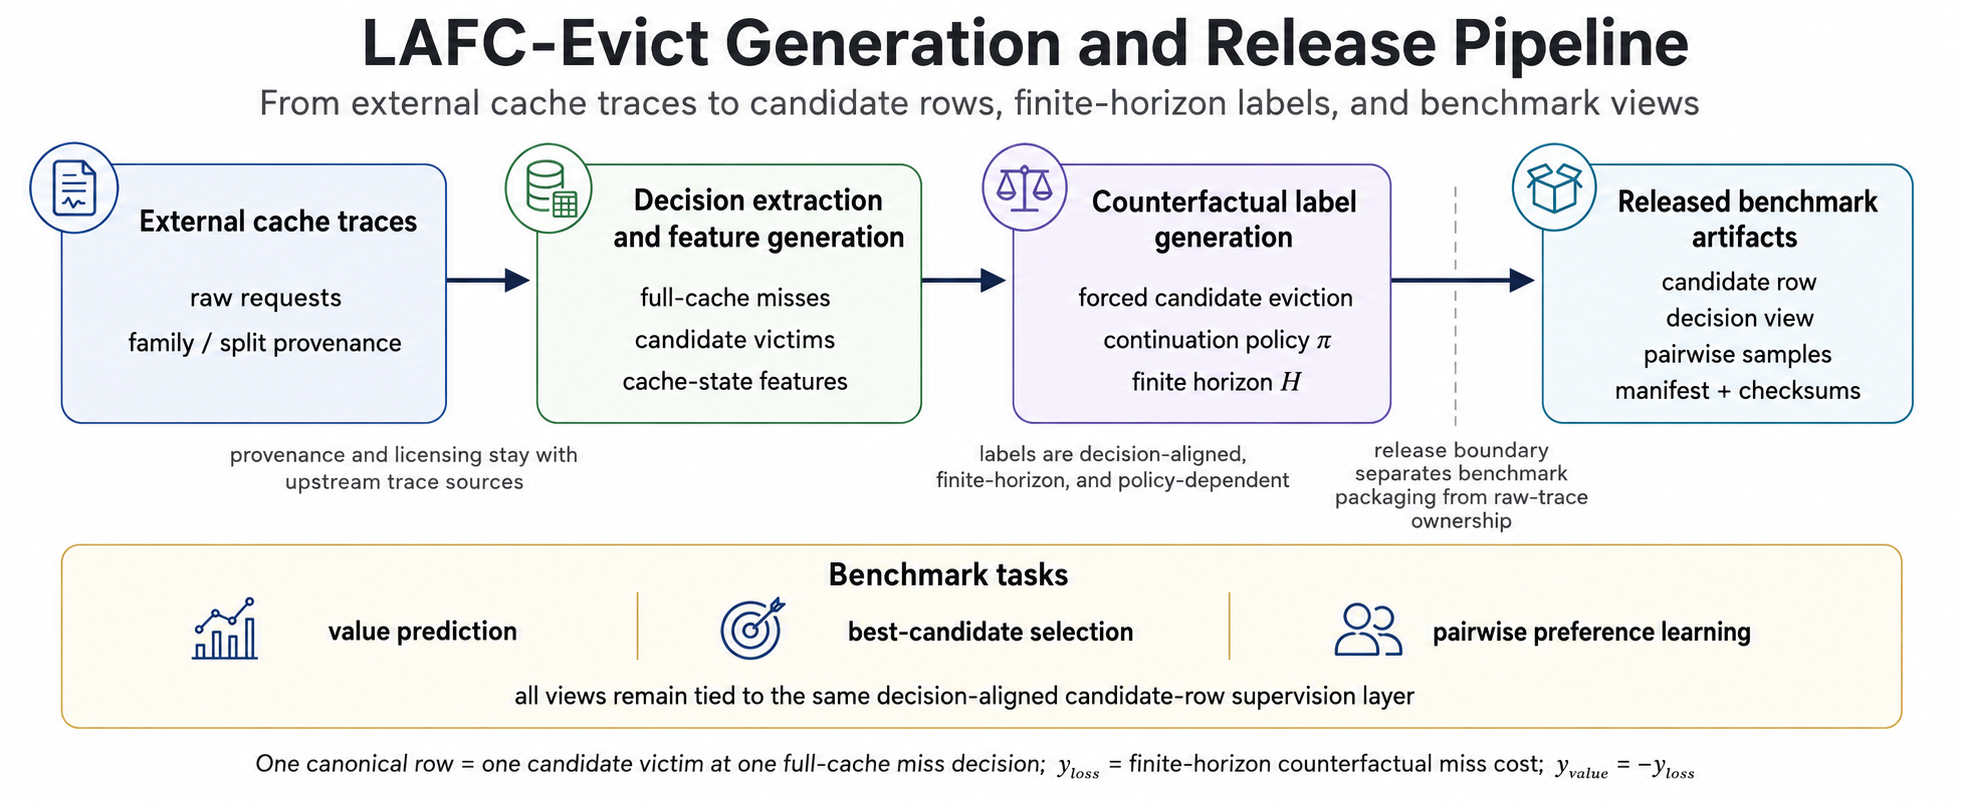
\includegraphics[width=\textwidth]{../../64BDAA68-CBD4-4E8E-800B-467D62C0D9DE.png}
  \caption{LAFC-Evict generation and release pipeline. External cache traces are converted into decision-level candidate rows, finite-horizon counterfactual labels, and released benchmark views for value prediction, best-candidate selection, and pairwise preference learning.}
  \label{fig:pipeline}
\end{figure}

The evaluated dataset covers five trace families -- \texttt{cloudphysics}\footnote{\texttt{cloudphysics} is a historical internal family identifier retained in project manifests, evidence records, and code for reproducibility. The underlying workload is Alibaba Cloud's Elastic Block Storage production block-storage trace, not the VMware/CloudPhysics dataset. Reader-facing prose below refers to this workload as ``alibaba-block.''},
\texttt{metacdn}, \texttt{metakv}, \texttt{twemcache}, and
\texttt{wiki2018} -- chosen to span a CDN workload, a key-value workload,
two additional production-derived workloads, and one intentionally
included negative/control workload (wiki2018; Sections~\ref{sec:characterization}
and~\ref{sec:mechanisms} show why it degenerates and treat that as a
useful, explained result rather than a benchmark defect). Two further
families, \texttt{brightkite} and \texttt{citibike}, are excluded from the
open release subset for redistribution reasons; this is a release-packaging
boundary, not a claim that the underlying generated corpus is limited to
five families. This five-family evaluated corpus is itself broader than
the currently downloadable public v0.3 subset, which packages only the
wiki2018 slice; the Data Availability statement details the redistribution
clearance and hosting status of the other four evaluated families. Not
every family appears in every split (e.g.\ metacdn
contributes train/validation but no test decisions); split assignment is
produced upstream of this release package and is normalized and validated,
not assigned, here.

The evaluation in this paper is organized to satisfy four requirements:
\begin{enumerate}[leftmargin=*]
  \item \textbf{Decision alignment.} Preserve within-decision candidate
  competition rather than treating candidates as i.i.d.\ points.
  \item \textbf{Task multiplicity.} Support pointwise (candidate-level),
  decision-level, and pairwise views of the same underlying supervision.
  \item \textbf{Closed-loop grounding.} Evaluate the offline labels
  against actual closed-loop cache-policy behavior rather than presenting
  them as self-validating (Sections~\ref{sec:closed-loop}
  and~\ref{sec:linkage}).
  \item \textbf{Reproducibility.} Expose validated, checksummed evidence
  for every reported number (Section~\ref{sec:release-validation}).
\end{enumerate}

\begin{table}[tbp]
  \centering
  \small
  \caption{Canonical evaluation protocol and workload specifications per trace family. Every family has release capacities of $\{32, 64, 128, 256\}$ and horizons of $\{4, 8, 16\}$, while closed-loop evaluation focuses on capacities $\{32, 128\}$.}
  \label{tab:evaluation-protocols}
  \begin{tabularx}{\textwidth}{@{}l P{0.13\textwidth} c c L c@{}}
    \toprule
    Family & Workload & Splits & CL Split & Scored Window & Warm-up / Init \\
    \midrule
    \texttt{alibaba-block} & Block Storage & train/val/test & test & 2 chunks (8,192 req.) & Warm \\
    \texttt{metacdn} & CDN Cache & train/val & validation & 3 chunks (20,480 req.) & Warm \\
    \texttt{metakv} & Key-Value & train/val/test & test & 1 chunk (4,096 req.) & Cold Start \\
    \texttt{twemcache} & Memcached & train/val/test & test & 2 chunks (8,192 req.) & Warm \\
    \texttt{wiki2018} & Wikipedia & train/val/test & test & 1 chunk (4,096 req.) & Warm \\
    \bottomrule
  \end{tabularx}
\end{table}


The canonical workload and evaluation parameters are summarized in Table~\ref{tab:evaluation-protocols}. When reading and interpreting the results, the following trace-specific design nuances should be kept in mind:
\begin{itemize}[leftmargin=*]
  \item \textbf{MetaCDN Validation Status:} Tier-1 closed-loop evidence for MetaCDN uses validation-window chunks because no Tier-1 test-split chunks are available at these capacities. The separate learned-policy campaign evaluates MetaCDN under its own independent held-out protocol.
  \item \textbf{MetaKV Cold Start:} MetaKV is evaluated starting from an empty cache (a cold start) with no leading unscored warm-up, whereas the other four workload families continuous-warmup from preceding unscored trace prefixes.
  \item \textbf{Wiki2018 Negative Control:} Wiki2018 is a deterministic zero-reuse negative-control workload where all candidate eviction options result in identical miss costs (100\% tie-degenerate, zero random regret), acting as a baseline verification of cache boundaries.
\end{itemize}

Detailed release characteristics, including candidate scale (277M rows) and exact split breakdowns, are provided in Appendix~\ref{sec:appendix-release-tables} (Tables~\ref{tab:dataset-scale} and~\ref{tab:split-counts}).

\section{Experimental Methodology}
\label{sec:experimental-methodology}

This section consolidates the methodological choices used across every
result reported in Sections~\ref{sec:characterization}--\ref{sec:continuation}
so that scope and caveats are stated once rather than scattered.

\textbf{Workloads, capacities, horizons.} All results use the five
families defined in Section~\ref{sec:benchmark-design}
(alibaba-block, metacdn, metakv, twemcache, wiki2018). Offline
target-discriminativeness results (Section~\ref{sec:characterization}) span
all four evaluated capacities (32, 64, 128, 256) and all three horizons
($H\in\{4,8,16\}$). Closed-loop, linkage, mechanistic, and continuation
results (Sections~\ref{sec:closed-loop}--\ref{sec:continuation}) are
reported at capacities 32 and 128 only -- this is the scope of the Tier-1
production closed-loop evaluation on which all three later sections
depend, not a data-availability limitation, and it is stated here once
rather than repeated in each section.

\textbf{Split terminology and two family-specific caveats.} ``test''
denotes a temporally held-out scoring window; ``validation'' denotes a
window used during earlier development that is not temporally held out in
the same sense. Two caveats apply and recur throughout the paper: (i)
\textbf{metacdn's closed-loop evidence is validation-window evidence, not
test-window}, for both of its evaluated capacities; every result that
includes metacdn should be read with this in mind, and Section~\ref{sec:linkage}
reports what changes if metacdn is excluded. (ii) \textbf{metakv is the
only family whose scored window begins at an empty cache} (a cold start,
identifiable from the identity $\mathit{evictions} = \mathit{misses} -
\mathit{capacity}$ holding exactly for metakv and no other family);
Section~\ref{sec:mechanisms} discusses this as a plausible, not
established, contributor to metakv's one policy-ranking exception.

\textbf{Policies and seeds.} Closed-loop replay is evaluated for LRU, MRU,
SIEVE (all deterministic, one run each), and random (20 CRN seeds, seeds
0--19; mean and per-seed standard deviation reported). SIEVE has no
offline counterpart in the labels described in Section~\ref{sec:label-generation}
and is therefore closed-loop-only evidence throughout -- it is not part of
any offline-vs-closed-loop correspondence claim, but is still reported as
a closed-loop reference point (Section~\ref{sec:closed-loop}).

\textbf{Offline metrics.} Per decision: all-tied fraction, unique-winner
fraction, mean/median optimal-set fraction, decision-weighted random-optimal
probability, and random regret (mean and tail percentiles), all computed
per (family, capacity, horizon) stratum before any pooling
(Section~\ref{sec:characterization}).

\textbf{Closed-loop metrics.} Miss ratio per (family, capacity, policy),
and, for random, its across-seed mean and standard deviation; relative
miss-ratio difference vs.\ LRU is reported as the primary comparison
statistic (Section~\ref{sec:closed-loop}).

\textbf{Offline$\leftrightarrow$closed-loop linkage metrics.} Sign
concordance between the offline regret gap and the closed-loop miss-ratio
gap (MRU-vs-LRU and random-vs-LRU only, since these are the two pairs with
both an offline and a closed-loop side), plus Pearson/Spearman/Kendall
correlation between the two gaps' magnitudes, computed per horizon on the
$n=10$ (family, capacity) cells (Section~\ref{sec:linkage}). $n=10$ is
small and is treated as such throughout: correlations are reported with
their exact $n$, never as population-scale claims.

\textbf{Continuation-sensitivity metrics.} Optimal-set Jaccard overlap,
cross-continuation regret (in misses), and strict-reversal fraction,
comparing the canonical LRU-continuation label against MRU- and
mean-random-continuation (10 CRN seeds) relabelings of the same decisions,
on a pre-registered, stratified 5,000-primary + 500-diagnostic decision
sample at capacities 32 and 128, plus a full-population MRU census over
all five families, capacities 32/64/128/256, and horizons 4/8/16
(Section~\ref{sec:continuation}). The primary statistical unit here is
the \emph{decision} (not the candidate row or the continuation seed):
every reported sampled-study statistic is a decision-level cluster
statistic, and the two reported bootstrap confidence intervals (one per
continuation policy; Section~\ref{sec:continuation}) resample at the
decision level; the MRU census is reported as a complete population
enumeration, not an inferential sample.

\textbf{Tie-aware analysis.} Every metric above that could be silently
distorted by ties (optimal-set membership, pairwise preference,
concordance) is computed with ties as a first-class outcome rather than
broken arbitrarily; Section~\ref{sec:background}'s worked example shows
the base case this generalizes from.

\textbf{Provenance and validation strategy.} Every number in this paper
traces to a validated evidence record. The closed-loop, linkage,
mechanistic, and continuation analyses were checked by reproducible scripts
and, where applicable, by independent recomputation of headline values
(Section~\ref{sec:release-validation}). No number in this paper is read
from a partial or unvalidated intermediate run; the full-population MRU
continuation census is used only after complete-record validation and an
independent recheck.

\section{Counterfactual Label Generation}
\label{sec:label-generation}

The benchmark label is defined on candidate victims rather than on completed policies. Let $r_1, r_2, \ldots$ denote a request sequence, and let $t$ index a request $r_t$ that misses when the cache is full. Write $S_t^{-}$ for the cache state immediately before the eviction choice; the candidate set $C_t = S_t^{-}$ is every resident object, so $|C_t|$ equals the cache capacity (32, 64, 128, or 256 objects in the evaluated release), counted in objects rather than bytes, with upstream object sizes not separately modeled. For any candidate $c \in C_t$, consider the intervention that evicts $c$, admits the missed request into the freed slot, and then follows a fixed continuation policy $\pi$ for the next $H$ requests, resolving every subsequent miss according to $\pi$; in the evaluated release, $\pi$ is LRU continuation rather than a Belady/offline-optimal rule. The resulting finite-horizon counterfactual loss counts those subsequent misses, so every miss contributes unit cost:
\[
\begin{aligned}
L_{t,H}^{\pi}(c)
&=
\#\{\tau \in \{t+1, \ldots, t+H\} : \\
&\qquad r_{\tau} \text{ misses in the induced trajectory}\}.
\end{aligned}
\]
The release stores this quantity as \texttt{y\_loss}, and it stores the corresponding value label as \texttt{y\_value} $= -\texttt{y\_loss}$. The triggering miss at time $t$ is common to all candidates and is therefore not the decision-discriminating part of the label.

Both columns are retained in the schema, but they are not independent
information: \texttt{y\_value} is a deterministic sign-flip of
\texttt{y\_loss}, computed by the same generation step. The two exist
because downstream modeling code is written against either a
minimization convention (\texttt{y\_loss} as a cost/regret target, the
convention used throughout the rest of this paper and the more directly
interpretable of the two -- a count of extra misses) or a maximization
convention (\texttt{y\_value} as a value/utility target, convenient for
argmax-based candidate selection or value-function-style formulations).
This paper treats \texttt{y\_loss} as canonical and uses
\texttt{y\_value} only where a specific baseline is more naturally stated
as a maximization, never reporting the same statistic under both names.

This label has two consequences for the paper. First, it creates a common numerical target for regression-style benchmark tasks. Second, it induces structured decision-level objects. For a fixed decision $(t, S_t^{-}, C_t)$, the benchmark-optimal candidate set is
\[
C_t^{\star} = \arg\min_{c \in C_t} L_{t,H}^{\pi}(c),
\]
and the per-candidate regret is
\[
\Delta_{t,H}^{\pi}(c) = L_{t,H}^{\pi}(c) - \min_{c' \in C_t} L_{t,H}^{\pi}(c').
\]
These quantities define best-candidate selection targets, pairwise preferences, and tie structure within a decision.

This supervision is a generated counterfactual label family, not an upstream annotation. It is finite-horizon, not asymptotic. It is tied to a continuation policy, not a universally optimal control objective. The label is therefore decision-aligned for the benchmarked eviction choice, but it is not an offline-optimal label in the sense of solving the full future control problem. These boundaries are central to the scientific positioning of the paper.

\section{Dataset Schema and Views}
\label{sec:schema-views}

Each released row corresponds to exactly one candidate victim at exactly
one full-cache-miss decision: which trace and split it came from, the
cache configuration (capacity, horizon), which decision it belongs to,
the candidate's identity, its label (\texttt{y\_loss}, the finite-horizon
counterfactual miss cost defined in Section~\ref{sec:label-generation},
and its sign-flipped alias \texttt{y\_value}), and a set of request/
candidate/cache features. Table~\ref{tab:schema-summary} lists the full
column groups; this section describes only the two derived views built on
top of these rows.

Grouping candidate rows by decision identifier gives the \emph{decision
view}: candidate count, minimum loss, the set of optimal candidates, tie
count, and regret summary statistics for that decision (this is exactly
the aggregation illustrated by hand in Section~\ref{sec:background}).
Comparing candidate pairs within a decision and ordering them by
\texttt{y\_loss} gives the \emph{pairwise view}, with ties when losses are
equal; the evaluated open release ships a capped 1,000,000-row pairwise
sample rather than the full pairwise view. The three views are layered
projections of the same underlying decisions -- candidate rows are the
atomic supervised objects, the decision view groups them, and the pairwise
sample keeps selected within-decision comparisons -- not three separate
sources of ground truth.

\begin{table}[t]
  \caption{Compact summary of candidate-row schema groups and derived-view fields.}
  \label{tab:schema-summary}
  \centering
  \footnotesize
  \begin{tabularx}{\columnwidth}{@{}P{0.31\columnwidth}L@{}}
    \toprule
    Column group & Notes \\
    \midrule
    Decision metadata & family, capacity, horizon, split, IDs \\
    Candidate identity & candidate page ID \\
    Labels & \texttt{y\_loss}, \texttt{y\_value} \\
    Feature groups & request, candidate, cache, disagreement, rate \\
    Derived decision fields & tie and regret summaries \\
    Derived pairwise fields & A/B labels and regret differences \\
    \bottomrule
  \end{tabularx}
\end{table}

\section{Release Construction and Validation}
\label{sec:release-validation}

The release packages existing generated candidate rows into a benchmark
artifact without requiring raw traces, and validates that package before
any number in this paper is computed from it. Validation checks schema
completeness, split normalization, presence of the selected families and
absence of blocked ones, duplicate candidates within a decision,
consistency of decision metadata, decision-view count consistency, and
checksums (Table~\ref{tab:artifact-layout} summarizes the package
components these checks cover). This validation is itself part of the
contribution: a released benchmark is only as trustworthy as the checks
that produced it, so we treat it as reproducible evidence rather than an
implementation detail.

\begin{sloppypar}
The evaluated open-release snapshot passed metadata repair, the full
verification suite, publication-bundle validation, and end-to-end release
validation, all via reproducible scripts rather than manual inspection.
This is validation of the release package itself; it does not claim that
public hosting or DOI assignment is complete, and superseded status notes
are never treated as evidence in their own right.
\end{sloppypar}

\begin{table}[t]
  \centering
  \footnotesize
  \caption{Release-package layout using release-relative paths for the evaluated benchmark snapshot.}
  \label{tab:artifact-layout}
  \begin{tabularx}{\columnwidth}{@{}P{0.31\columnwidth}L@{}}
    \toprule
    artifact & relative\_path \\
    \midrule
    candidate rows & data/candidate\_rows/ \\
    decision view & data/decision\_view/decision\_view.parquet \\
    pairwise sample & data/pairwise\_sample/pairwise\_sample.parquet \\
    release manifest & metadata/release\_manifest.json \\
    checksums & metadata/checksums.sha256 \\
    \bottomrule
  \end{tabularx}
\end{table}


\subsection{Provenance of the evaluation results in this paper}

Beyond the released dataset artifact above, every result reported in
Sections~\ref{sec:characterization}--\ref{sec:continuation} traces to an
independently frozen, gate-validated analysis artifact, each with its own
committed scripts, provenance record, and (where applicable) an
independent second code path that recomputes headline numbers and
requires exact agreement: the target-discriminativeness audit, the Tier-1
closed-loop production evidence (14/14 validity gates; a byte-verified
evidence freeze recording the SHA256 of every output file both before and
after freezing), the offline$\leftrightarrow$closed-loop linkage analysis,
the mechanistic workload analysis, and the continuation-policy sensitivity
pilot and full sampled study (prelaunch LRU-equivalence gate;
post-completion validity gates; an independent recheck script requiring
$10^{-9}$ numerical agreement with the primary analysis), plus the
full-population MRU continuation census (60/60 chunks, 2{,}363{,}286
decision-horizon records, 30/30 validity gates, independent recheck
passed). All six are scripted, reproducible, and checked into the
repository alongside this manuscript as compact evidence artifacts.

\textbf{Two label sources must not be conflated.} The canonical labels
evaluated throughout this paper always use LRU continuation
(Section~\ref{sec:label-generation}). The MRU and random \emph{relabelings}
computed for the continuation-sensitivity study
(Section~\ref{sec:continuation}) exist only to measure sensitivity and are
never treated elsewhere as the canonical label.

\textbf{The population-scale MRU continuation census is frozen evidence.}
The census (run \texttt{20260914T042528Z\_1a29e773a113}) is complete,
validated, and independently rechecked; its manifest and validation report
are committed to the repository. The raw 1.6 GB census output is preserved
separately outside this
manuscript branch; the manuscript imports only compact summaries,
validation reports, manifests, and Figure~\ref{fig:continuation-robustness}
source data.

\textbf{A known, unresolved provenance limitation.} The exact historical
commit provenance of the full-release label generator is incomplete. This
does not affect the validity of the frozen analysis artifacts above, each
of which independently
records its own generation provenance, but it means the full historical
lineage of the generator code itself predating those artifacts is not
completely reconstructable from repository history alone.

\section{Benchmark Tasks and Baselines}
\label{sec:tasks-baselines}

\lafc\ supports four benchmark tasks from one release.

\paragraph{Candidate-level value prediction.}
Predict \texttt{y\_loss} or \texttt{y\_value} from a single candidate row. This is a pointwise task over the canonical benchmark unit and measures how well a model predicts finite-horizon counterfactual eviction quality for one candidate at one decision.

\paragraph{Best-candidate selection.}
Given all candidate rows for one decision, identify a member of the minimum-loss set. This task can be framed as ranking or decision-level classification and connects most directly to the actual cache-eviction choice because it evaluates whether a method selects a benchmark-optimal victim within that decision.

\paragraph{Pairwise preference prediction.}
Predict whether candidate A is better than candidate B within the same decision, where ``better'' means lower \texttt{y\_loss} or equivalently higher \texttt{y\_value}. This task uses the pairwise view or the shipped pairwise sample and provides a simpler learning interface for within-decision preference modeling. Because equal losses induce ties, reports using this task need to state explicitly whether evaluation includes tie rows, excludes them, or maps them to a separate class. Within the shipped pairwise sample, the A/B assignment is randomized by a deterministic hash over stable decision and pair-identity fields (\texttt{orientation\_method: deterministic\_hash\_v1}), not by candidate-identifier ordering, so the non-tie \texttt{label\_a\_better}/\texttt{label\_b\_better} split is balanced (about 49.8\%/50.2\%) rather than reflecting a construction-induced directional imbalance.

\paragraph{Candidate-label distribution characterization.}
Summarize the empirical label surface without training a predictive model. This characterization task studies distributions of \texttt{y\_loss}, \texttt{y\_value}, regret, tie frequency, and decision ambiguity across families, capacities, horizons, and splits. It is descriptive rather than competitive, but it is important for understanding benchmark difficulty and for interpreting downstream task results.

The empirical scope of this paper remains intentionally narrow. Rather than presenting a large model bake-off, we report lightweight baselines that can be executed directly from the committed release views and that establish reproducible reference points for later work.

\begin{sloppypar}
The current results surface covers three such references. A linear regression baseline over candidate rows predicts \texttt{y\_loss} from released features. It is intentionally weak: test MAE is 3.8739 with RMSE 4.7152 and $R^2=0.0026$, and the validation-split $R^2$ is slightly negative ($-0.0506$). Using that same linear score for within-decision selection nevertheless provides a reproducible decision-level floor. On the pairwise task, the earlier random and majority non-tie results remain useful sanity checks, but by themselves they do not test whether the released candidate features contain decision-relevant signal.
\end{sloppypar}

To probe that question without changing the released benchmark schema, we build an augmented feature view for evaluation only by joining released candidate-side features back onto the capped shipped pairwise sample. This produces a pairwise-sample-backed evaluation surface rather than a full-pairwise-universe-backed one, and no full quadratic pairwise materialization is performed. The shipped sample used throughout this paper is the canonical
regenerated pairwise sample (SHA256 prefix
\texttt{1d770c69\ldots9eda02}, full digest and provenance in the
accompanying reproducibility artifact),
not the historical, noncanonical sample that a stale six-column
decision-selection key produced in an earlier release artifact; the
regenerated sample's tie-count balance below (near-50/50 non-tie split) is
itself evidence of this, since the historical sample's non-tie rows were
heavily skewed (about 6{,}134 vs.\ 113{,}898) in a way traceable to the
key bug, not to the underlying label distribution. It is itself tie-heavy: 878,262 of its 1,000,000 rows (87.8\%) are exact ties, leaving 121,738 non-tie rows evaluated below. Ties remain common and are reported here as part of the label-surface characterization rather than discarded. Table~\ref{tab:pairwise-feature-baselines} reports six non-tie pairwise baselines on that 121,738-row surface: the random and majority sanity checks, 1-D LRU-score and predictor-score models, a pairwise baseline induced by the released pointwise linear \texttt{y\_loss} regressor, and a logistic regression over released feature differences.

The resulting evidence is stronger than the earlier sanity checks alone. The logistic feature-difference model is the strongest pairwise baseline, reaching 0.9660 accuracy with 0.0824 log loss on the non-tie subset of the shipped sample. The linear-score and LRU-score baselines also outperform the random and majority checks, which indicates that the released candidate features retain decision-relevant signal for pairwise preference prediction. These numbers nevertheless warrant conservative interpretation. They improve the empirical benchmark evidence without changing the released candidate-row, decision-view, or shipped pairwise artifacts, and they do not support full-universe or online-policy claims.

The best-candidate evaluator groups candidate rows by the canonical
9-column decision key and reports 2,363,286 decisions, an exact match
with the decision view (Section~\ref{sec:benchmark-design}). A cheap
decision-level floor computed directly from the decision view shows why
this match matters for interpretation: a uniform-random selector's
expected optimal-selection rate is 0.9912 with expected regret 0.0088,
both more favorable than the linear-score selector's observed 0.8753
optimal-selection rate and 0.1251 mean regret, purely because of the tie
density documented in Section~\ref{sec:characterization} -- not because
the linear score underperforms a stronger baseline. Headline
selection-rate and regret numbers should therefore always be read
alongside this random floor rather than in isolation.

\begin{table}[t]
  \centering
  \footnotesize
  \caption{Pairwise-sample-backed summary statistics for the shipped sample view.}
  \label{tab:pairwise-sample-stats}
  \begin{tabularx}{\columnwidth}{@{}P{0.34\columnwidth}L@{}}
    \toprule
    statistic & value \\
    \midrule
    pairwise rows & 1,000,000 \\
    split breakdown & test=102,024; train=737,896; val=160,080 \\
    family breakdown & wiki2018=250,872; alibaba-block=245,336;\newline
    metakv=190,584; twemcache=169,064;\newline
    metacdn=144,144 \\
    unique decisions represented & 118,635 \\
    label distribution & a\_better=60,673; b\_better=61,065;\newline
    tie=878,262 \\
    A/B orientation method & deterministic\_hash\_v1 (randomized, not lexicographic) \\
    \bottomrule
  \end{tabularx}
\end{table}


\begin{table}[t]
  \centering
  \footnotesize
  \caption{Feature-based pairwise baselines on the non-tie subset (121,738 of 1,000,000 rows) of the shipped pairwise sample, evaluated after the A/B orientation fix (deterministic hash-based randomization, not lexicographic ordering). An evaluation-only augmented feature view joins released candidate features back to the capped sample. Results are pairwise-sample-backed rather than full-pairwise-universe-backed, and no full quadratic pairwise materialization is performed.}
  \label{tab:pairwise-feature-baselines}
  \begin{tabularx}{\columnwidth}{@{}P{0.24\columnwidth}LP{0.16\columnwidth}P{0.14\columnwidth}@{}}
    \toprule
    baseline & feature source / model type & accuracy & log loss \\
    \midrule
    random non-tie & random-label sanity check & 0.5006 & 0.6931 \\
    majority non-tie & empirical majority-class sanity check & 0.5016 & 0.6931 \\
    LRU-score pairwise & 1-D logistic on LRU-score difference & 0.9225 & 0.2426 \\
    predictor-score pairwise & 1-D logistic on predictor-score difference & 0.5016 & 0.6931 \\
    linear-score pairwise & logistic on pointwise linear-score difference & 0.9490 & 0.1161 \\
    logistic feature difference & logistic regression on released feature differences & 0.9660 & 0.0824 \\
    \bottomrule
  \end{tabularx}
\end{table}


\begin{table}[t]
  \caption{Benchmark task definitions and representative evaluation outputs.}
  \label{tab:task-definitions}
  \centering
  \footnotesize
  \begin{tabularx}{\columnwidth}{@{}P{0.22\columnwidth}P{0.20\columnwidth}L@{}}
    \toprule
    Task & Inputs & Representative outputs \\
    \midrule
    Value regression & candidate rows & MAE, RMSE, and optional rank correlation between predicted and observed values \\
    Best-candidate selection & decision groups & Top-1 accuracy against the benchmark-optimal set and mean realized regret relative to the best available candidate \\
    Pairwise preference & pairwise rows from one decision & Accuracy or ROC-AUC, with tie handling stated explicitly and non-tie-only reporting marked when used \\
    Label characterization & candidate or decision aggregates & Histograms, quantiles, tie rates, regret summaries, and per-family/capacity/horizon breakdowns \\
    \bottomrule
  \end{tabularx}
\end{table}

\section{Empirical Characterization}
\label{sec:characterization}

The empirical characterization emphasizes benchmark structure rather than a large model bake-off. The release metadata establish the scale and heterogeneity of the benchmark, and the released candidate-row summaries add full label-distribution reporting without changing that focus.

Across 277,995,072 candidate rows, \texttt{y\_loss} has mean 7.7561, standard deviation 4.6542, and 5/25/50/75/95th percentiles of 2/4/7/11/16. The corresponding \texttt{y\_value} summary mirrors those values by sign, as expected from the benchmark definition. The resulting label surface is broad but still bounded by the finite horizon, which keeps both candidate-level regression errors and decision-level regret interpretable. Table~\ref{tab:decision-breakdown}'s exactly equal horizon counts (787,762 rows at each of horizons 4, 8, and 16) reflect the same underlying full-cache-miss decisions relabeled at each configured horizon, whereas its capacity counts correspond to genuinely different full-cache-miss events produced by replaying each trace at each cache size; pooled statistics in this paper therefore mix horizons and capacities and should be read as aggregate release summaries rather than per-configuration results.

The same result summaries also show that the simple linear-score selector often lands in the benchmark-optimal set even though its underlying value regression is weak. That combination is useful descriptive context for later benchmark users: the release is not trivial, but a lightweight heuristic already clears a reproducible lower bar. The evaluator's grouped decision count now matches the manifest-backed decision-view count exactly (Table~\ref{tab:label-selection-summary}); an earlier decision-key bug that double-counted a small number of decisions has been fixed and reconciled. Because the dataset is heavily tied at the decision level, a uniform-random selector's expected optimal-selection rate and regret are included alongside the linear-score selector's observed metrics so that headline numbers are not read in isolation from tie density.

\begin{table}[!h]
  \centering
  \footnotesize
  \caption{Decision-view-backed benchmark composition by family, capacity, horizon, and split.}
  \label{tab:decision-breakdown}
  \begin{tabularx}{\columnwidth}{@{}P{0.22\columnwidth}L@{}}
    \toprule
    dimension & counts \\
    \midrule
    trace\_family & wiki2018=598,560; alibaba-block=576,219;\newline
    metakv=454,053; twemcache=397,494;\newline
    metacdn=336,960 \\
    capacity & 32=613,314; 64=599,172;\newline
    128=582,678; 256=568,122 \\
    horizon & 4=787,762; 8=787,762; 16=787,762 \\
    split & test=242,418; train=1,746,882; val=373,986 \\
    \bottomrule
  \end{tabularx}
\end{table}


\begin{table}[t]
  \centering
  \footnotesize
  \caption{Decision-view-backed candidate-count statistics. These values summarize the number of candidates per decision in the preserved release.}
  \label{tab:candidate-count-stats}
  \begin{tabular}{@{}lrrrr@{}}
    \toprule
    group & min & med & mean & max \\
    \midrule
    overall & 32 & 64 & 117.63 & 256 \\
    alibaba-block & 32 & 64 & 118.35 & 256 \\
    metacdn & 32 & 64 & 117.12 & 256 \\
    metakv & 32 & 64 & 119.52 & 256 \\
    twemcache & 32 & 64 & 111.52 & 256 \\
    wiki2018 & 32 & 64 & 119.85 & 256 \\
    \bottomrule
  \end{tabular}
\end{table}


\begin{table}[t]
  \centering
  \footnotesize
  \caption{Candidate-label and best-candidate-selection summaries from validated result records.}
  \label{tab:label-selection-summary}
  \begin{tabularx}{\columnwidth}{@{}P{0.50\columnwidth}L@{}}
    \toprule
    statistic & value \\
    \midrule
    candidate rows summarized & 277,995,072 \\
    \texttt{y\_loss} mean / std & 7.7561 / 4.6542 \\
    \texttt{y\_loss} q05 / q25 / q50 / q75 / q95 & 2 / 4 / 7 / 11 / 16 \\
    \texttt{y\_value} mean / std & -7.7561 / 4.6542 \\
    \texttt{y\_value} q05 / q25 / q50 / q75 / q95 & -16 / -11 / -7 / -4 / -2 \\
    manifest-backed decision rows & 2,363,286 \\
    best-candidate evaluator decision count & 2,363,286 (exact match) \\
    \midrule
    \multicolumn{2}{@{}l}{\textit{all decisions (secondary, ecological view)}} \\
    best-candidate optimal-selection rate & 0.8753 \\
    best-candidate regret mean / median / max & 0.1251 / 0 / 3 \\
    random-selector expected optimal-selection rate & 0.9912 \\
    random-selector expected regret & 0.0088 \\
    \midrule
    \multicolumn{2}{@{}l}{\textit{discriminative decisions only (primary selector-quality view)}} \\
    discriminative decisions (opt.\ candidate count $<$ candidate count) & 764,282 (32.34\%) \\
    best-candidate optimal-selection rate & 0.6145 \\
    best-candidate mean regret & 0.3867 \\
    random-selector expected optimal-selection rate & 0.9729 \\
    random-selector expected regret & 0.0273 \\
    \bottomrule
  \end{tabularx}
\end{table}


\section{Closed-Loop Policy Evaluation (RQ2, part 1)}
\label{sec:closed-loop}

\begin{sloppypar}
Section~\ref{sec:characterization} characterizes the offline target.
This section reports the actual closed-loop cache-policy behavior it will
be compared against in Section~\ref{sec:linkage} (Table~\ref{tab:tier1-closed-loop}). Source: Tier-1
production closed-loop evaluation (repository path
\texttt{analysis/closed\_loop\_tier1\_evidence\_20260914/}; RUN\_ID
\texttt{20260914T023445Z\_8a4cd32402a1}; 14/14 validity gates
passed; 230/230 planned executions complete, 0 failed). Scope: 5 families
$\times$ 2 capacities (32, 128) $\times$ 4 policies (LRU, MRU, random-mean
over 20 seeds, SIEVE~\cite{zhang2024sieve}), per
Section~\ref{sec:experimental-methodology}.
\end{sloppypar}

\begin{table}[t]
  \centering
  \footnotesize
  \caption{Tier-1 closed-loop production evaluation: LRU miss ratio and relative miss-ratio difference vs.\ LRU for MRU, mean-random (20 seeds), and SIEVE. Source: \texttt{analysis/closed\_loop\_tier1\_evidence\_20260914/} (230/230 complete, 14/14 gates passed). MetaCDN is validation-window evidence; all other families are test-window. Negative values mean the policy beats LRU.}
  \label{tab:tier1-closed-loop}
  \begin{tabularx}{\columnwidth}{@{}llrrrrr@{}}
    \toprule
    family & cap. & LRU miss ratio & MRU $\Delta$ & random $\Delta$ & SIEVE $\Delta$ & random std \\
    \midrule
    metacdn      & 32  & 0.5792 & +47.37\% & +5.38\% & +0.81\%  & 0.0013 \\
    metacdn      & 128 & 0.5490 & +54.93\% & +2.98\% & +0.36\%  & 0.0014 \\
    twemcache    & 32  & 0.7511 & +27.12\% & +4.19\% & +8.47\%  & 0.0025 \\
    twemcache    & 128 & 0.6205 & +52.98\% & +7.78\% & +15.29\% & 0.0023 \\
    metakv       & 32  & 0.7410 & +10.02\% & +0.47\% & +0.03\%  & 0.0011 \\
    metakv       & 128 & 0.7290 & +8.57\%  & $-$2.07\% & $-$4.22\% & 0.0015 \\
    cloudphysics & 32  & 0.9836 & +1.65\%  & +0.28\% & +0.20\%  & 0.0010 \\
    cloudphysics & 128 & 0.9561 & +4.48\%  & +0.85\% & +1.44\%  & 0.0014 \\
    wiki2018     & 32  & 1.0000 & 0.00\%   & 0.00\%  & 0.00\%   & 0.0000 \\
    wiki2018     & 128 & 1.0000 & 0.00\%   & 0.00\%  & 0.00\%   & 0.0000 \\
    \bottomrule
  \end{tabularx}
\end{table}


\textbf{LRU is the best policy in 9 of 10 cells.} The sole exception is
metakv/cap128, where SIEVE (miss ratio 0.6982) beats LRU (0.7290) by
4.22\% relative -- the only cell in the entire evaluation where a
non-LRU policy wins outright. \textbf{MRU is the worst policy in every
non-degenerate cell}, by a wide margin (relative miss-ratio increase over
LRU ranging from 1.65\% at alibaba-block/cap32, a near-zero-signal regime,
up to 54.93\% at metacdn/cap128). \textbf{Random-seed variability is small
relative to policy gaps} throughout: the largest random-policy standard
deviation observed is 0.0025 (twemcache/cap32), an order of magnitude
below the smallest genuine policy gap reported in the table.

\textbf{wiki2018 is a complete, exact tie across every policy}: miss ratio
1.0 for LRU, MRU, SIEVE, and every one of random's 20 seeds, at both
capacities, with random's standard deviation exactly 0.0. This is not
approximate degeneracy -- it is byte-for-byte identical across all 4
policies and 20 seeds. Section~\ref{sec:mechanisms} shows this follows
deductively from zero reuse events in the scored window, not as a
statistical artifact of this particular closed-loop run.

\textbf{alibaba-block is a near-tie regime at both capacities}: every
policy's relative gap to LRU stays under 4.5\%, an order of magnitude
smaller than metacdn's or twemcache's gaps. \textbf{The metakv/cap128 cell is the one genuine exception to "LRU
dominates"}, and there both SIEVE (miss ratio 0.6982) and random-mean
(approximately 0.7137, relative gap $-2.07\%$) beat LRU (0.7290), while
MRU remains worst; Section~\ref{sec:mechanisms} investigates, but does not
fully resolve, why. metacdn's results should be read as validation-window
evidence throughout (Section~\ref{sec:experimental-methodology});
twemcache's are test-window.

No universal middle-of-the-pack ranking is claimed for SIEVE vs.\ random:
SIEVE beats random-mean at metacdn and metakv/cap32, but random-mean beats
SIEVE at twemcache (both capacities), alibaba-block (both capacities), and
metakv/cap128 -- the relative order of these two policies is
family-dependent, not fixed. Only one ordering statement holds across
every non-degenerate cell: \textbf{MRU is worst everywhere}. Among this
four-policy comparator set, LRU is best in 9 of 10 cells and falls only as
low as third place, at metakv/cap128, in the tenth.

\subsection{Robustness to an Expanded Comparator Set}
\label{sec:expanded-comparators}

\begin{sloppypar}
LRU/MRU/random/SIEVE is a deliberately small, diagnostic comparator set,
not a full policy-landscape comparison (Section~\ref{sec:related-work}
surveys the broader landscape of classical and modern replacement
policies \lafc\ interfaces with). To test whether the conclusions above
are an artifact of that narrow set, we add three representative stronger
baselines under the identical Tier-1 protocol (same 5 families, same
capacities 32/128, same scored windows and trace hashes): \textbf{ARC}
\cite{megiddo2003arc} (adaptive recency/frequency), \textbf{LIRS}
\cite{jiang2002lirs} (inter-reference-recency), and \textbf{S3-FIFO}
\cite{yang2023s3fifo} (modern lightweight FIFO-family, using its own
published default ratios, not tuned to any trace). All three are
deterministic, reference C implementations from libCacheSim, the same
simulator family as the SIEVE reference implementation already used in
Table~\ref{tab:tier1-closed-loop}, independently validated before
production use (hand-derived tiny-trace tracing for ARC, a cross-check of
the library's own LRU engine against this manuscript's already-trusted
LRU implementation, and a scan-resistance property check). A fourth
candidate, W-TinyLFU, was pre-registered but dropped after validation
found its reference implementation non-functional at capacity 32 under
its own published default configuration; see this experiment's
\texttt{COMPARATOR\_PROTOCOL.md} for the full pre-registration and this
finding.
\end{sloppypar}

\input{tables/table_problem5_expanded_closed_loop}

\begin{figure}[t]
  \centering
  
\includegraphics[width=\columnwidth]{figures/figure_problem5_policy_spread_vs_discriminativeness.pdf}
  \caption{Closed-loop policy spread (max$-$min miss ratio across all 7
  policies) versus offline discriminative fraction at $H=16$, one point per
  family$\times$capacity cell. The offline-discriminativeness$\leftrightarrow$
  closed-loop-separation association (Section~\ref{sec:linkage}) is
  essentially unchanged when the policy landscape is expanded ($r=0.96$
  with the original 4-policy spread vs.\ $r=0.96$ with the expanded
  7-policy spread, $n=10$).}
  \label{fig:policy-spread}
\end{figure}

Under the expanded 7-policy set, LRU is strictly the best policy in 4 of
10 cells (down from 9 of 10 among the original four). However, four of
the six cells where a new policy edges out LRU do so by less than 3.2\%
relative miss ratio -- comparable in size to gaps this manuscript already
treats as near-ties elsewhere (e.g.\ alibaba-block's sub-4.5\% policy
gaps) -- so most of this apparent reordering reflects fine-grained
jockeying among already-close policies, not a qualitative reversal. The
one cell with a clearly large margin is the already-known exception,
\textbf{metakv/cap128}, where the gap to LRU widens under the broader set
(S3-FIFO's miss ratio is 8.07\% below LRU's, versus SIEVE's previously
reported 4.22\%); no new family/capacity cell crosses that magnitude. LRU
remains worst-case-safe and near-best almost everywhere; it is not
displaced as the practical default, but it is no longer accurate to say it
wins outright in nearly every cell once the comparator set is broadened.
Most importantly for RQ3, the link between offline discriminativeness and
closed-loop policy separation is not an artifact of the narrow original
comparator set: it is essentially identical whether policy separation is
measured across 4 or 7 policies (Figure~\ref{fig:policy-spread}).

\section{Offline$\leftrightarrow$Closed-Loop Correspondence (RQ2, part 2)}
\label{sec:linkage}

This section answers the second half of RQ2 -- does the offline candidate
ranking from Section~\ref{sec:characterization} correspond to the
closed-loop behavior in Section~\ref{sec:closed-loop}? -- and, jointly
with the horizon comparison below, RQ3's horizon question. Source:
\texttt{analysis/closed\_loop\_offline\_linkage\_20260914/}, computed with
two independent code paths in numerical agreement. \textbf{SIEVE has no
offline counterpart} (Section~\ref{sec:label-generation} defines labels
only for the continuation-policy family LRU/MRU/random) and is therefore
excluded from every comparison in this section; only MRU-vs-LRU and
random-vs-LRU are compared.

\textbf{RQ-CL1 (rank agreement).} At $H=16$, across the 10 family$\times$capacity
cells: MRU-vs-LRU agrees in sign (offline regret-gap sign matches
closed-loop miss-ratio-gap sign) in 7 of 10 cells, disagrees in 1, and is
tied on both sides (wiki2018) in 2; random-vs-LRU agrees in 6, disagrees
in 2, ties in 2. The discordant cells are always the same two:
\textbf{alibaba-block/cap32} (discordant for both pairs -- offline regret
gaps there are $-0.0027$ and $-0.0007$, i.e.\ barely non-zero on the
offline side too) and \textbf{metakv/cap128} (discordant for random-vs-LRU
only -- offline says random is very slightly worse than LRU, $+0.0013$
regret gap, while closed-loop shows random modestly beating LRU, $-0.015$
miss-ratio gap; Section~\ref{sec:closed-loop} additionally notes SIEVE
also beats LRU there). Excluding wiki2018's two trivially-tied cells,
concordance among the 8 non-degenerate cells is not manufactured by
wiki2018's automatic agreement: dropping wiki2018 still leaves the same
two discordant cells and the same qualitative picture.

\textbf{RQ-CL2 (gap-magnitude correspondence).} At $H=16$: MRU-vs-LRU
Pearson $r=0.835$ (Spearman $\rho=0.915$, Kendall $\tau=0.773$);
random-vs-LRU $r=0.755$ ($\rho=0.829$, $\tau=0.591$). Figure~\ref{fig:linkage-scatter}
shows both relationships directly, with the two discordant cells
annotated rather than hidden. These correlations rest on only 8--10
independent (family, capacity) points and are reported with that $n$
attached everywhere; they are not treated as population-scale estimates.

\begin{figure}[t]
  \centering
  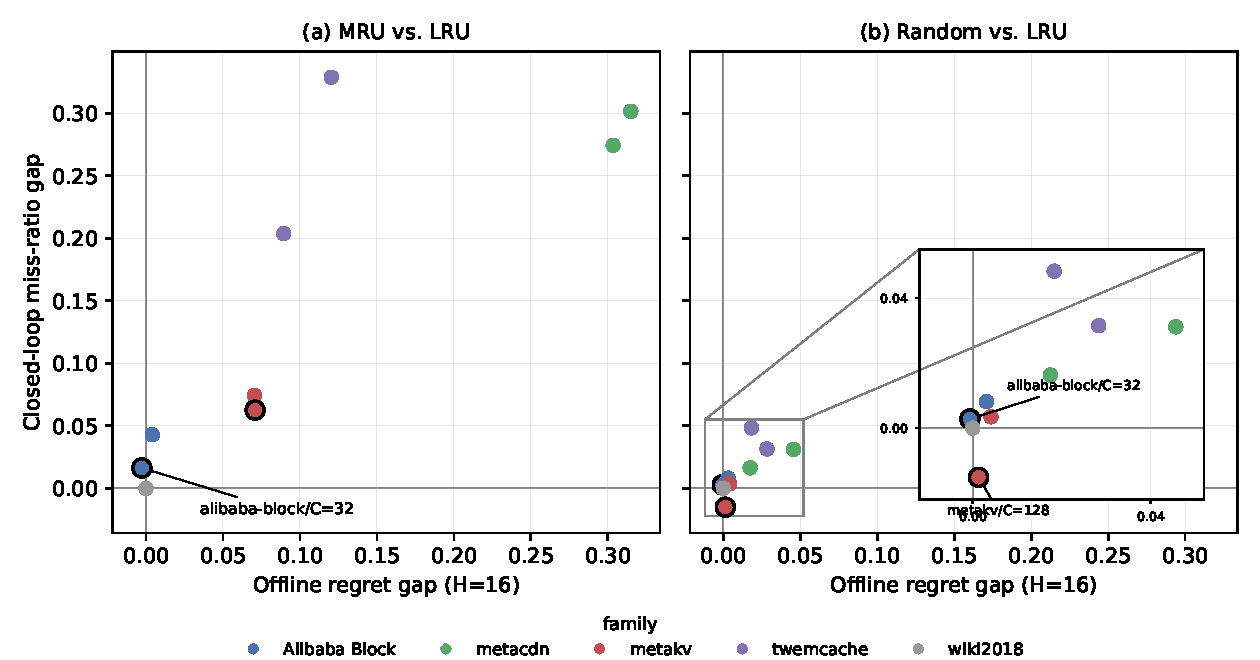
\includegraphics[width=\columnwidth]{figures/figure3_linkage_scatter.pdf}
  \caption{Offline regret gap vs.\ closed-loop miss-ratio gap, H=16, MRU-vs-LRU
  and random-vs-LRU. Reproducible from
  \texttt{paper/performance\_evaluation/scripts/figures/make\_figure3\_linkage\_scatter.py}
  against \texttt{outputs/rq\_cl2\_scatter\_data.csv}.}
  \label{fig:linkage-scatter}
\end{figure}

\textbf{RQ-CL3 (workload/capacity dependence).} metacdn and twemcache are
the strong-agreement, most-discriminative-offline regimes and also show
the largest closed-loop policy separation; alibaba-block is a
weak/ambiguous regime where the offline gap is close enough to zero that
its sign is not robust; metakv/cap128 is the one reversal regime; wiki2018
is degenerate on both sides, exactly, confirming it as a clean negative
control. An exploratory (not pre-registered) correlation between offline
discriminativeness ($1-\text{all-tied fraction}$) and closed-loop
$|\text{MRU}-\text{LRU}|$ separation, across all 10 cells at $H=16$, gives
Pearson $r=0.968$ -- Section~\ref{sec:mechanisms} traces this to a shared
underlying trace-locality property rather than treating it as a
coincidence.

\textbf{RQ-CL4 (horizon).} $H=16$ wins or ties on every magnitude-sensitive
statistic across every sensitivity slice tested (primary, excluding
wiki2018, test-window-only), for both pairs. The coarse concordant/
discordant/tied counts are \emph{identical} at $H=4$, $H=8$, and $H=16$
(the same two cells are discordant regardless of horizon); horizon changes
the \emph{strength} of the correspondence (the correlation coefficients
above), not which cells agree in sign. The differences between horizons
are modest in absolute terms ($r=0.746$ at $H=4$ to $r=0.835$ at $H=16$
for MRU-vs-LRU) and $n=8$--10 per horizon is small, but the pattern is
consistent and not cherry-picked.

\textbf{Answer to RQ2/RQ3.} Offline and closed-loop policy orderings agree
in the large majority of workload/capacity regimes where the offline
signal itself is not near zero, with two specific, characterized
exceptions; $H=16$ gives the strongest, though modest, alignment among the
three horizons tested. This is a bounded, evidenced claim, not a universal
predictive-validity claim for the offline labels.

\section{Mechanistic Workload Analysis (RQ3, part 2)}
\label{sec:mechanisms}

Sections~\ref{sec:characterization} and~\ref{sec:linkage} show
\emph{that} discriminativeness and offline$\leftrightarrow$closed-loop
agreement vary by workload; this section asks \emph{why}, using only
existing trace-only and closed-loop artifacts (no new simulation). Source:
repository path
\texttt{analysis/\allowbreak closed\_\allowbreak loop\_\allowbreak mechanistic\_\allowbreak analysis\_\allowbreak 20260914/}.
Classifications follow the source report's own discipline exactly:
\textsc{directly observed} (a deductive or exactly-reproduced fact),
\textsc{consistent with mechanism} (plausible, structurally supported, not
proven), and \textsc{causally established} (reserved for one deductive
result below). No claim here is upgraded beyond its source classification.

\textbf{Capacity-scale reuse correlates with both discriminativeness and
closed-loop separation.} Trace-derived LRU hit rate (an exact,
capacity-scale reuse measure, computed independently of the labels)
correlates with offline discriminativeness at $r=0.83$ and with
closed-loop $|\text{MRU}-\text{LRU}|$ separation at $r=0.90$ (pooled
$n=10$). Figure~\ref{fig:locality} shows both relationships directly.
This is an $n=10$, exploratory finding, consistent with but not
independent evidence from RQ-CL3's own exploratory correlation
(Section~\ref{sec:linkage}) -- the same underlying trace property is
driving both.

\begin{figure}[t]
  \centering
  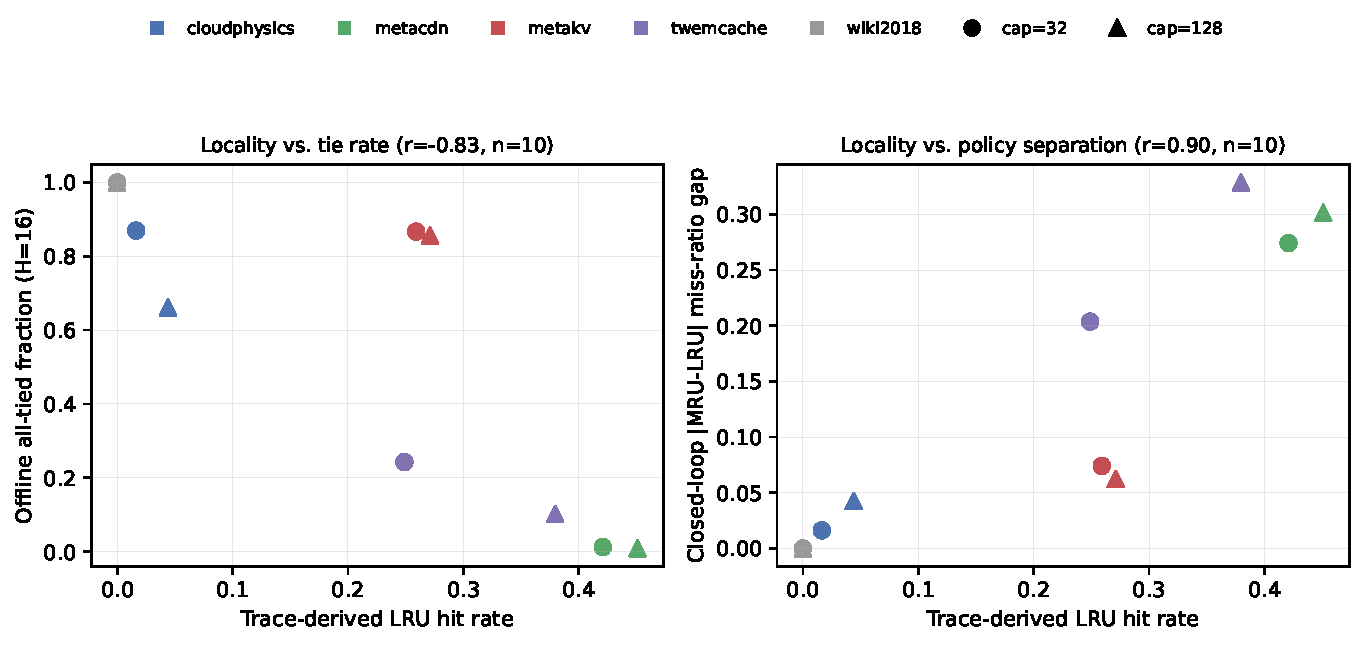
\includegraphics[width=\columnwidth]{figures/figure4_locality.pdf}
  \caption{Trace-derived LRU hit rate vs.\ offline discriminativeness
  (left) and closed-loop policy separation (right), $n=10$ family$\times$capacity
  cells. Reproducible from
  \texttt{paper/performance\_evaluation/scripts/figures/make\_figure4\_locality.py}
  against \texttt{outputs/mechanism\_comparison.csv}.}
  \label{fig:locality}
\end{figure}

\textbf{alibaba-block/cap32 is near-zero signal.} Only 17.5\% of window requests are
reuses at all; of those, only 9.4\% fall within stack distance 32. The
trace-only predicted LRU hit rate ($0.175 \times 0.094 = 1.6\%$) exactly
reproduces the observed Tier-1 LRU hit rate (134/8192 = 1.64\%). The
offline regret gaps there ($-0.0027$, $-0.0007$) are tiny on a scale where
metacdn's own MRU-LRU gap is over 100$\times$ larger. The
Section~\ref{sec:linkage} discordance at this cell is exactly what a
coin-flip-scale signal would produce.

\textbf{metakv/cap128 remains a bounded exception.} metakv's reuse-distance median is short (2, comparable to
metacdn's 3) but its tail is markedly heavier: reuse-within-32 is only
0.574, rising to just 0.600 by distance 128 -- a narrow, 2.6-percentage-point
``boundary zone'' sitting almost exactly at the tested capacities, where a
recency-strict policy (LRU) and a second-chance policy (SIEVE) can
plausibly diverge. metakv's cold-start scoring window
(Section~\ref{sec:experimental-methodology}) is a second, independently
real structural property of this same cell. \textbf{Neither is shown to be
the cause}: no per-request SIEVE or random trajectory log exists in the
frozen artifacts to isolate which property (or their interaction, or
neither) produced the reversal, and the source analysis states this
explicitly rather than forcing a resolution.

\textbf{twemcache's random-over-SIEVE ordering is not explained by
existing data.} twemcache has the strongest ``small hot set plus long
tail'' bimodal signature in the dataset (longest novel streak 3; reuse
distance p10=3 but p75=7379), which would naively predict SIEVE's
second-chance admission should help -- but the observed result is the
opposite (SIEVE loses to random at both capacities). Existing trace-only
data can describe this structure but cannot explain the direction of the
outcome; the source analysis classifies any ``SIEVE benefits from
bimodality'' story here as \textsc{not supported} by the data, and this
paper does not repeat that story.

\textbf{wiki2018 (\textsc{causally established}): the one exception to the
paper's general classification discipline, and deliberately so.} Zero
reuse events occur in the scored window ($n_{\text{reuse}}=0$ across all
4096 requests, every one a first-ever occurrence over the full 50{,}000-request
trace). Since a hit requires a repeated reference to an already-resident
item, miss ratio $=1.0$ for every policy is a mathematical certainty given
zero reuse events, not a statistical tendency -- an existence proof from a
directly counted quantity, which is why this one result is classified
\textsc{causally established} while every other mechanism in this section
is not.

\section{Continuation-Policy Sensitivity (RQ4)}
\label{sec:continuation}

The canonical labels use LRU as the continuation policy after a forced eviction. RQ4 asks whether the optimal-candidate set and regret ordering are materially changed if followed by a different continuation policy. Table~\ref{tab:linkage-continuation-summary} summarizes this sensitivity evidence.

\begin{table}[t]
  \centering
  \footnotesize
  \caption{Offline$\leftrightarrow$closed-loop correspondence and sampled continuation-policy robustness, summarized. Top: H=16 concordance/correlation across the 10 family$\times$capacity cells (\texttt{analysis/closed\_loop\_offline\_linkage\_20260914/}). Bottom: sampled continuation study, Set C (discriminative-under-LRU, $n{=}6597$ primary-sample decisions; \texttt{analysis/continuation\_policy\_sensitivity\_full\_20260914/}), capacities 32/128 only --- population-scale evidence pending census validation.}
  \label{tab:linkage-continuation-summary}
  \begin{tabularx}{\columnwidth}{@{}Lrr@{}}
    \toprule
    \multicolumn{3}{@{}l}{\textit{Offline$\leftrightarrow$closed-loop, H=16 (n=10 cells; SIEVE excluded, no offline counterpart)}} \\
    \midrule
    metric & MRU-vs-LRU & random-vs-LRU \\
    \midrule
    Concordant / discordant / tied (of 10) & 7/1/2 & 6/2/2 \\
    Pearson $r$ & 0.835 & 0.755 \\
    Spearman $\rho$ & 0.915 & 0.829 \\
    Kendall $\tau$-b & 0.773 & 0.591 \\
    \midrule
    \multicolumn{3}{@{}l}{\textit{Sampled continuation robustness, Set C, by capacity}} \\
    \midrule
    metric & cap.\ 32 & cap.\ 128 \\
    \midrule
    MRU median / mean Jaccard & 1.000 / 0.9958 & 1.000 / 0.9999 \\
    MRU mean cross-cont.\ regret & 0.0018 & 0.0001 \\
    MRU strict reversal fraction & 2.7$\times10^{-5}$ & 0.0 \\
    random median / mean Jaccard & 1.000 / 0.7251 & 1.000 / 0.8522 \\
    random mean cross-cont.\ regret & 0.0463 & 0.0197 \\
    random strict reversal fraction & 1.0$\times10^{-3}$ & 1.5$\times10^{-6}$ \\
    \midrule
    \multicolumn{3}{@{}l}{\textit{Sampled continuation robustness, Set C, by horizon (both capacities pooled)}} \\
    \midrule
    metric & H=4 & H=16 \\
    \midrule
    MRU median Jaccard & 1.000 & 1.000 \\
    random median Jaccard & 1.000 & 0.881 \\
    \bottomrule
  \end{tabularx}
\end{table}


\textbf{Sampled MRU/random study.} A pre-registered sampled study evaluates 5{,}500 decisions at capacities 32 and 128. By the pre-registered informative-stratum (Set C) rule, both MRU and mean-random continuation classify ROBUST. MRU is very close to LRU: Set-C mean Jaccard is 0.9958 (cap 32) and 0.9999 (cap 128). Mean-random continuation is more perturbing but still robust: mean Jaccard is 0.7251 (cap 32) and 0.8522 (cap 128). 

\textbf{Full-population MRU census.} The full-population MRU census extends the MRU result to all five families and capacities 32, 64, 128, and 256. Across all 2{,}363{,}286 decision-horizon units, mean optimal-set Jaccard is 0.99941, median Jaccard is 1.0, and 98.69\% of records have exact Jaccard 1. Strict preference reversals are extremely rare ($1.87\times10^{-7}$). 

Because 67.31\% of records are all-tied under both LRU and MRU, the pre-registered decisive stratum is Set C (764{,}282 records). Here, mean Jaccard is 0.99846, median Jaccard is 1.0, and mean cross-continuation regret is 0.000638 misses. Since wiki2018 contributes no Set-C records, this is not inflated by the degenerate negative control.

\textbf{Scope and limitations.} Sensitivity is largest at small capacities and long horizons, but remains small in absolute terms. The worst Set-C cell (alibaba-block/cap32/$H=16$) yields mean Jaccard 0.9804 and median 1.0, satisfying the pre-registered robustness criterion. These results substantiate robustness within the evaluated scope (sampled random at capacities 32/128, and full-population MRU). They do not establish population-scale random-continuation robustness or guarantee that arbitrary deployed policies would preserve the ordering.

\begin{figure}[t]
  \centering
  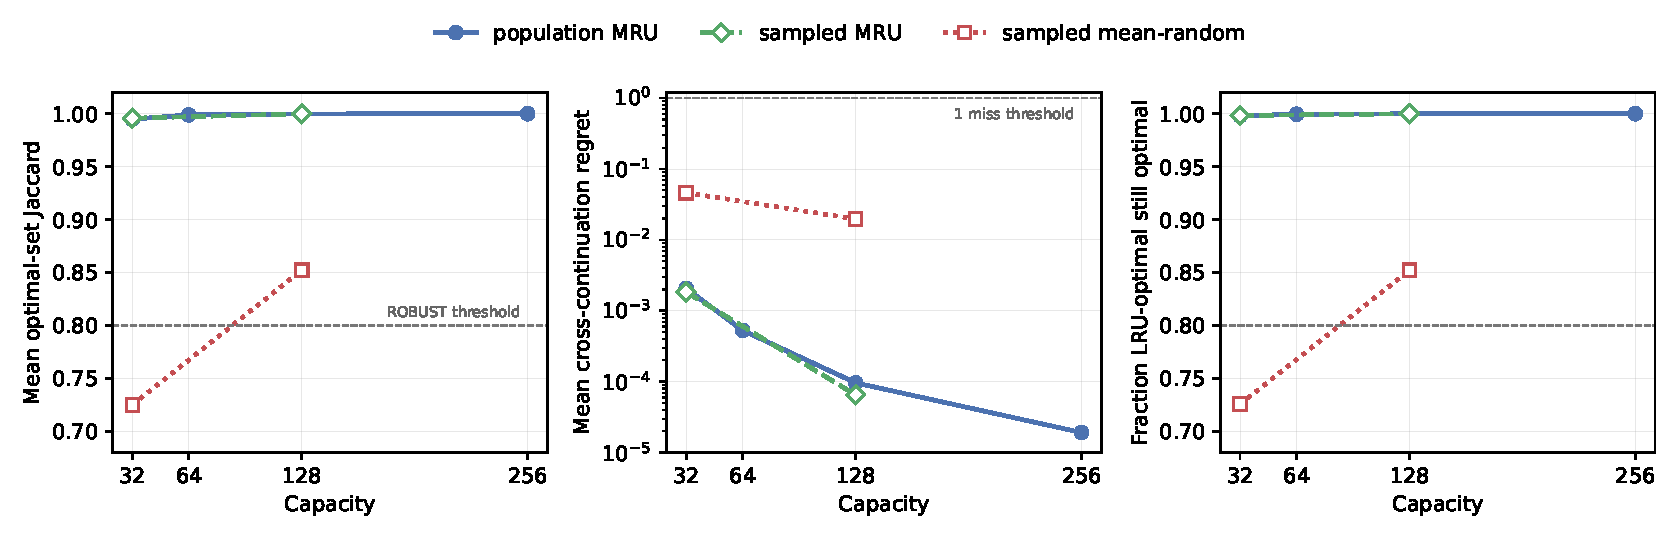
\includegraphics[width=\columnwidth]{figures/figure5_continuation_robustness.pdf}
  \caption{Continuation-policy sensitivity in the pre-registered
  informative stratum (Set C). Sampled MRU and mean-random evidence covers capacities 32 and 128 only;
  full-population MRU evidence covers capacities 32--256.}
  \label{fig:continuation-robustness}
\end{figure}
\FloatBarrier

\section{Practical Implications (RQ5)}
\label{sec:practical-implications}

This section synthesizes the preceding results into guidance for using finite-horizon counterfactual supervision.

\textbf{When should the offline signal be trusted?} Most directly in workload/capacity regimes with high capacity-scale reuse, identifiable before closed-loop replay via a high trace-derived LRU hit rate or low all-tied fraction. In this dataset, this corresponds to metacdn- and twemcache-like regimes, where offline discriminativeness and closed-loop agreement are strongest.

\textbf{When is caution warranted?} In near-zero-signal regimes (e.g., alibaba-block/cap32), small offline regret gaps may flip signs without reflecting genuine disagreement. Caution is also needed when interpreting cold-start evaluation windows (metakv) or validation-only regimes (metacdn). A high tie rate is itself informative: it identifies where policy comparison is fundamentally unresolvable by this label family (e.g., wiki2018), preventing researchers from hunting for non-existent signal.

\textbf{Why still run closed-loop evaluation?} The offline/closed-loop association is real but bounded, resting on $n=10$ cells with at least one unexplained exception (metakv/cap128). Offline-label results are complementary diagnostics and cannot replace closed-loop performance claims.

\textbf{How should continuation-policy assumptions be interpreted?} As a tested robustness property with real limits. The labels are highly robust to MRU continuation at population scale, and acceptably robust to random continuation in the validated sample. This supports the use of canonical LRU-continuation labels in evaluated regimes, but does not imply continuation choice is universally irrelevant.

\section{Discussion}
\label{sec:discussion}

\textbf{What LAFC-Evict enables.} A reusable, candidate-level, finite-horizon
counterfactual supervision surface, materialized once from real traces and
usable across value-regression, best-candidate-selection, and pairwise
formulations (Sections~\ref{sec:background}--\ref{sec:tasks-baselines})
without every study re-deriving its own labels from raw traces
(Section~\ref{sec:related-work} situates this against prior learned-cache
work, most of which derives labels internally and non-reusably).

\textbf{What the evaluation reveals, beyond the surface itself.} Four
findings that only emerge from evaluating the surface against closed-loop
behavior, not from describing the surface alone: the target's
discriminativeness is workload-structured, not incidental
(Section~\ref{sec:characterization}); that structure is explained, not
just observed, by a single trace-level property, capacity-scale reuse
(Section~\ref{sec:mechanisms}); offline and closed-loop policy orderings
agree in most, not all, informative regimes, with the exceptions
identified rather than smoothed over (Section~\ref{sec:linkage}); and the
canonical LRU-continuation assumption is robust, with quantified limits,
at the capacities tested (Section~\ref{sec:continuation}).

\textbf{Why the negative/degenerate regimes are scientifically useful, not
an embarrassment.} wiki2018's complete degeneracy and alibaba-block/cap32's
near-zero offline signal are both, in this paper, explained results
(Section~\ref{sec:mechanisms}), not unexplained anomalies. A benchmark
whose degenerate cases are mechanistically understood is more trustworthy
in its non-degenerate claims than one that reports only favorable cases;
this is the paper's answer to the historical criticism that the target's
tie-heaviness was previously stated but not investigated.

\textbf{Offline surrogate evaluation vs.\ closed-loop performance.} This
paper's position, supported by Sections~\ref{sec:linkage}
and~\ref{sec:closed-loop}, is that the offline surrogate is a genuine,
partially-validated predictor of closed-loop policy separation in
identifiable regimes, and that this relationship is itself the
contribution -- not a claim that the surrogate can replace closed-loop
evaluation. The two exceptions found (alibaba-block/cap32,
metakv/cap128) are not edge cases invented for balance; they were
identified by the same symmetric procedure that found the 8 agreeing
cells, and metakv/cap128 in particular remains only partially understood
even after dedicated mechanistic analysis (Section~\ref{sec:mechanisms}).

\textbf{Continuation robustness as currently validated.} The robustness
finding in Section~\ref{sec:continuation} is deliberately reported with
its exact scope attached: sampled MRU and mean-random continuation at
capacities 32/128, and full-population MRU continuation at capacities
32/64/128/256. Within that scope, the LRU continuation used for label
generation is not driving the target ordering to a practically meaningful
degree: Set-C median Jaccard remains 1.0, mean cross-continuation regret
is below 0.001 misses in the population MRU census, and capacities 64/256
do not reveal hidden sensitivity. The result does not say that every
stateful deployed continuation policy would preserve the same ordering;
it says the tested alternatives did, with random tested only in the
validated sample.

\textbf{Methodological limitations that shape every result above} are
collected in Section~\ref{sec:limitations} rather than repeated here;
Section~\ref{sec:characterization}'s target-discriminativeness numbers,
Section~\ref{sec:linkage}'s small $n$, and Section~\ref{sec:continuation}'s
continuation-policy scope are the three limitations most load-bearing for
the claims in this discussion specifically.

\section{Limitations, Ethics, and Reuse}
\label{sec:limitations}

\lafc's labels and evaluation have several important constraints, and the
practical guidance in Section~\ref{sec:practical-implications} should be
read together with them rather than instead of them.

First, the main label is a finite-horizon, continuation-policy-specific
counterfactual miss cost, not an offline-optimal label for the full future
control problem. Good performance on this label does not automatically
imply online deployment gains, which is exactly why
Sections~\ref{sec:closed-loop} and~\ref{sec:linkage} evaluate closed-loop
behavior directly rather than relying on the offline label alone.

Second, horizon-dependent results are scoped to the horizons actually
evaluated. Most manuscript analyses use the canonical released
$H\in\{4,8,16\}$ decision population; the matched long-horizon audit extends
only the discriminativeness characterization through
$H\in\{32,64,128\}$ on the same physical decision population.
It shows that longer horizons increase informativeness but do not remove
degeneracy: substantial all-tied mass persists at $H=128$, and wiki2018
remains fully tied. No result here covers $H>128$.

Third, the canonical labels use LRU continuation after a forced eviction.
The sampled MRU/random study and full-population MRU census in
Section~\ref{sec:continuation} support robustness only within their stated
scopes; random continuation is not validated at population scale, and no
experiment covers every deployment policy.

Fourth, the target is substantially tied (Section~\ref{sec:characterization}:
all-tied fraction 0.68, unique-winner fraction exactly 0.0). Support for
the benchmark's usefulness is conditional on decision informativeness, not
universal, and no result in this paper claims it generalizes beyond the
audited population. wiki2018 remains a fully degenerate negative control
at every capacity and horizon tested; Section~\ref{sec:mechanisms} proves
this follows deductively from zero reuse events, not as a statistical
property of the trace.

Fifth, the evaluated dataset uses unit-object, count-based capacities (32,
64, 128, or 256 objects) with unconditional admission of the requested
object. Variable object sizes, byte-weighted miss cost, latency-aware cost,
and dirty-write cost are not modeled by this label family, and admission
is never withheld. Claims in this paper should be read as scoped to this
abstraction and not generalized to byte-addressable or admission-gated
cache models without further evidence.

Sixth, closed-loop evidence carries two family-specific caveats stated in
full in Section~\ref{sec:experimental-methodology}: MetaCDN's evidence is
validation-window, not test-window; MetaKV's scored window begins at an
empty cache. Section~\ref{sec:mechanisms} discusses, without resolving,
whether the cold start plausibly contributes to MetaKV being the one
cell where LRU is not the best policy.

Seventh, a known data-generation issue remains open: in the audited
canonical data, the predictor-victim flag is identical to the LRU-victim
flag throughout, and related predictor, bucket, and confidence fields
include constant or placeholder values. This paper does not make any claim
that depends on those predictor fields being informative.

Eighth, benchmark reuse must preserve provenance distinctions. The release
exposes generated supervision and derived views, but it does not erase the
attribution, citation, or licensing requirements of the upstream raw traces
from which candidate rows were derived; those raw traces remain external
artifacts with their own governance constraints. The open subset is also
intentionally narrower than the full generated corpus for redistribution
reasons, and not every selected family appears in every split of the
evaluated release package. The exact generator commit for the full
historical release corpus is not completely reconstructed; this is
orthogonal to the audited evidence reported in this paper but is disclosed
here for reproducibility completeness.

Finally, this paper reports closed-loop results for LRU, MRU, random, and
SIEVE (Section~\ref{sec:closed-loop}), plus ARC, LIRS, and S3-FIFO under
the identical protocol (Section~\ref{sec:expanded-comparators}); it does
not report a closed-loop evaluation of any learned policy trained on these
labels, and the seven-policy set is still representative rather than
exhaustive -- CLOCK-Pro, GreedyDual-Size, and TinyLFU-family admission
variants beyond W-TinyLFU (excluded after a validation failure at capacity
32; see Section~\ref{sec:expanded-comparators}) remain untested here. A frozen pilot
(not the production Tier-1 evaluation reported here) previously found a
simple learned policy competitive with random and SIEVE but not with LRU
on one family, with the other pilot family blocked on the absence of an
independent test window; neither result is repeated or extended here, and
learned-policy closed-loop competitiveness remains future work rather than
a claim of this paper.

\section{Related Work}
\label{sec:related-work}

\begingroup
\sloppy

\subsection{Production Cache Workloads and Benchmark Traces}

Public traces and benchmark infrastructure provide the substrate for cache evaluation. The UMass Trace Repository and large-scale workload studies of key-value stores and Twemcache clusters demonstrate the value of realistic, heterogeneous request streams for systems research~\cite{umasstracerepo,atikoglu2012kvworkload,yang2020twemcache}. CacheLib further shows what that heterogeneity looks like from the inside of a single production caching engine, which must serve many such workloads simultaneously behind one shared implementation~\cite{berg2020cachelib}. More broadly, benchmark artifacts such as YCSB, OLTP-Bench, and the Join Order Benchmark made comparison easier by publishing reusable workloads, interfaces, and evaluation surfaces rather than one-off experiments~\cite{cooper2010ycsb,difallah2013oltpbench,leis2018job}. Cache-specific infrastructure such as libCacheSim and cache\_dataset further lowers the cost of trace-driven evaluation by providing high-performance simulation support and large open trace collections~\cite{libcachesim,cachedataset}. Existing trace libraries and simulators therefore supply essential raw material for cache studies, and some public artifacts even expose oracle-style features or procedural oracle policies. \lafc\ packages a different layer of supervision: for each full-cache miss decision and candidate victim, it releases finite-horizon counterfactual loss labels under a fixed continuation policy, together with decision-level and pairwise views.

Those distinctions matter because raw traces, workload studies, and simulator-oriented artifacts do not by themselves provide a reusable table of candidate-level finite-horizon counterfactual outcomes. \lafc\ is intended to complement that ecosystem rather than replace it. The artifact is useful precisely when a downstream user wants to study offline value regression, best-candidate selection, preference learning, or label-distribution analysis without first regenerating the same counterfactual rollouts from scratch.

\subsection{Learned Cache Replacement}

Recent learned-caching papers contribute online policies, policy-selection schemes, or learning frameworks rather than reusable supervised benchmarks, and they differ in what signal they learn from and at what granularity. LRB learns a relaxed Belady-style policy for CDN caching, and LHD instead models hit density directly for key-value caches~\cite{song2020lrb,beckmann2018lhd}. GL-Cache and 3L-Cache both target the efficiency and overhead profile of learned eviction, at group and object granularity respectively, so that a learned policy stays cheap enough to run inline~\cite{yang2023glcache,zhou2025threelcache}. LeCaR learns between replacement experts online~\cite{vietri2018lecar}, and CACHEUS extends that practical line with adaptive expert selection, giving both a mechanism for adjusting to changing workload regimes without full retraining~\cite{rodriguez2021cacheus}. Parrot uses imitation learning to approximate Belady-style replacement decisions from past accesses~\cite{liu2020parrot}, while Hawkeye and Mockingjay show how Belady-derived signals can guide deployable replacement policies in hardware caches~\cite{jain2016hawkeye,shah2022mockingjay}. MAT focuses on reducing the overhead of ML-guided eviction by using a heuristic filter around a learned module~\cite{yang2023mat}. ALPS emphasizes lightweight learned replacement and the practical cost of learning overheads~\cite{shahout2024alps}, while Feedforward Neural Networks for Caching is useful precisely because it questions whether heavier learned models are always justified~\cite{fedchenko2018fnncache}. HR-Cache extends the learned-caching line into edge delivery settings~\cite{torabi2024hrcache}.

HALP is a closer conceptual precedent worth singling out: it deploys a preference-learning eviction policy in production for YouTube's CDN, where a lightweight reward model is trained continuously from automated preference comparisons between candidate evictions -- a scheme the authors liken to reinforcement learning from feedback rather than supervised imitation of a fixed oracle~\cite{song2023halp}. This makes HALP the closest production system to \lafc's own pairwise derived view, but the two are not the same kind of artifact and should not be read as such. HALP's preference signal is generated and consumed online, as the primary training objective of a deployed policy; \lafc's pairwise view is instead a static, deterministic reformatting of candidate-level finite-horizon counterfactual labels that already exist independently of it (Section~\ref{sec:background}), released so pairwise/ranking-style methods can consume the same underlying supervision. \lafc\ does not claim any preference-learning contribution of its own -- HALP already demonstrates that preference signals are useful for eviction in production; \lafc's contribution is a reusable, decoupled label surface, not a new instance of preference learning. Baleen addresses a related but distinct problem, applying coordinated ML admission and prefetching -- rather than eviction -- to flash caches, and end-to-end optimizes for backend load rather than a per-candidate label~\cite{wong2024baleen}. It is included here as a reminder that objective design (what to admit and prefetch, not only what to evict) is a live and separate axis from the counterfactual-label problem \lafc\ addresses, not as a directly comparable eviction system.

Across all of these works, the primary contribution is a policy, a policy-selection scheme, or an online learning framework. By contrast, \lafc\ releases a static benchmark surface with candidate-level finite-horizon counterfactual labels, decision-view summaries, and a shipped pairwise sample for offline value regression, best-candidate selection, and preference-learning tasks. To our knowledge, we are not aware of a public artifact in this line that releases reusable per-candidate finite-horizon counterfactual supervision at this scale.

\subsection{Modern Heuristic and Non-Learning Eviction}

Classical cache-replacement work defines the policy landscape that any learned benchmark must eventually interface with. Belady's look-ahead policy remains the canonical offline reference point~\cite{belady1966study}. Offline analyses such as FOO/PFOO compute practical bounds on optimal caching with variable object sizes, but their artifacts target trace-level optimality analysis rather than a reusable per-decision, per-candidate supervised label surface~\cite{berger2018foopfoo}. Practical online policies then emphasize different signals: LIRS focuses on inter-reference recency~\cite{jiang2002lirs}, ARC adaptively balances recency and frequency~\cite{megiddo2003arc}, CLOCK-Pro revisits CLOCK-style replacement with stronger reuse sensitivity~\cite{jiang2005clockpro}, and GreedyDual-Size accounts for cost and size~\cite{cao1997greedydual}. TinyLFU and W-TinyLFU further show that admission and segmented cache management matter in modern software caches~\cite{einziger2017tinylfu,einziger2018wtinylfu}. More recent object-cache work shows that policy progress does not always come from heavier machinery: S3-FIFO argues that simple FIFO-based queueing can beat more elaborate baselines at scale~\cite{yang2023s3fifo}, and a companion analysis explains \emph{why} at a mechanism level -- lazy promotion and quick demotion, not queue discipline by itself, are what let FIFO-derived policies beat LRU-style recency tracking~\cite{yang2023lazypromotion}. SIEVE emphasizes turn-key deployability for web caches~\cite{zhang2024sieve} and, unlike S3-FIFO, is not only discussed here: it is one of the four closed-loop policy arms (alongside LRU, MRU, and random-mean) evaluated directly in Section~\ref{sec:closed-loop}. LAH revisits this same simple-heuristic family from the other direction: rather than proposing a new heuristic, it learns the \emph{parameters} of an existing one -- S3-FIFO, instantiated as S4-FIFO -- from a control plane decoupled from the data plane, reporting robustness and interpretability gains over both purely heuristic and heavier learned baselines~\cite{xia2026lah}. S3-FIFO, the lazy-promotion/quick-demotion analysis, and LAH are strong online comparison targets for future end-to-end studies, but only SIEVE among this group is evaluated here; \lafc\ does not claim a new eviction policy of its own. The contribution here is reusable supervision that can be used to train or diagnose such policies, not an online replacement rule that supersedes them.

\subsection{Learning-Augmented Caching Theory}

Another relevant line of work treats caching as an online problem augmented by predictions rather than as a supervised dataset, with provable robustness/consistency guarantees as the object of study rather than empirical miss ratio alone -- a genuinely different research question from the learned-from-data policies of the previous two subsections, and one \lafc\ is careful not to conflate with them. Competitive Caching with Machine Learned Advice and later learning-augmented caching results formalize how predictive advice can improve classical online algorithms while preserving worst-case robustness guarantees~\cite{lykouris2021mladvice,wei2020learningaugcache}. Robust Learning-Augmented Caching: An Experimental Study extends that line empirically, testing how the theoretical robustness/consistency trade-off behaves under realistic, imperfect predictors rather than only in the adversarial worst case~\cite{chledowski2021robustlac}, while Parsimonious Learning-Augmented Caching studies how much prediction access is really needed to retain the theoretical benefit~\cite{im2022parsimoniouslac}. LAH (previous subsection) sits at a practical bridge between this theoretical line and the learned-from-data policies above: it carries no formal competitive-ratio guarantee, but its explicit robustness and interpretability goals echo the same underlying concern that a learned or advice-driven component should degrade gracefully, not fail silently, when its signal is wrong~\cite{xia2026lah}. This perspective is complementary to \lafc\ rather than directly competing with it. Learning-augmented caching papers typically study online algorithms equipped with advice, predictor queries, and robustness objectives. By contrast, \lafc\ releases finite-horizon, continuation-policy-dependent counterfactual labels for every candidate within a decision. The artifact can train or diagnose predictors and eviction-scoring models before they are embedded into an online algorithm, and it supports value regression, best-candidate selection, pairwise preference learning, and label characterization from one release.

\subsection{Offline Surrogate Evaluation versus Deployed, Closed-Loop Behavior}

A methodological question this paper shares with several other applied-ML domains -- recommendation, autonomous driving, and reinforcement learning among them -- is whether an offline proxy metric, computed without deploying a policy, predicts that policy's actual closed-loop performance. Within caching specifically, Qiu, Yang, and Harchol-Balter give a sharp, caching-native instance of this same gap: increasing a cache's hit ratio can, past a certain point, \emph{decrease} end-to-end throughput and increase response time, because a higher hit ratio changes contention on the hit path itself~\cite{qiu2026hitratio}. That result targets a different offline/online pairing than this paper does -- cache hit ratio versus downstream system throughput, rather than finite-horizon counterfactual miss cost versus closed-loop miss ratio -- and this paper does not claim it studies the same quantity. What it establishes, directly and independently, is that a favorable cache-local metric need not imply favorable end-to-end system behavior -- exactly the caution that motivates treating Sections~\ref{sec:closed-loop} and~\ref{sec:linkage}'s closed-loop validation as necessary, rather than inferring closed-loop behavior from the offline labels alone. The broader cross-domain finding, outside caching, is the same in spirit: offline and online/closed-loop metrics correlate imperfectly and domain-specifically across recommendation, autonomous driving, and reinforcement learning, which is why closed-loop or online validation is treated as necessary rather than optional wherever it is feasible. This paper's Sections~\ref{sec:linkage} and~\ref{sec:closed-loop} pose the same question for finite-horizon counterfactual cache-eviction labels specifically, with a bounded, regime-characterized answer rather than a universal one; beyond the hit-ratio-versus-throughput result above, to the best of our knowledge we are not aware of prior work posing this offline-versus-closed-loop question for candidate-level cache-eviction supervision in particular. A broader cross-domain literature search for this methodological category outside caching (surrogate/offline-vs-closed-loop evaluation methodology as a topic in its own right, in recommendation/autonomous-driving/RL) remains only partially complete at the time of writing; see \texttt{docs/PE\_LITERATURE\_SEARCH\_GAPS.md} in the accompanying artifact for what was and was not verified.

\subsection{Positioning \lafc}

Public learning-to-rank collections such as LETOR and the Yahoo! Learning to Rank Challenge show how reusable labeled artifacts can organize a research community~\cite{liu2009ltr,qin2010letor,chapelle2011yahoo}. In that limited sense, \lafc\ is to learned cache eviction somewhat analogous to LETOR-style ranking corpora: a standardized candidate-level label surface reduces bespoke label generation and evaluation drift. The label design in \lafc\ also connects to counterfactual learning and ranking because each cache decision induces a candidate set, a minimum-loss subset, regret summaries, and a natural pairwise structure~\cite{swaminathan2015crm,li2011offlinecb,joachims2017unbiasedltr,saito2020pairwise}. Even so, \lafc\ is not simply a ranking dataset transplanted into systems. Its labels are tied to finite-horizon eviction outcomes under a specified continuation policy.

To state the boundary precisely, given the full literature surveyed above: \lafc\ does not claim to be the first to use future accesses for supervision (LRB, Parrot, and HALP all do so already); the first to support pairwise or preference-style modeling of cache decisions (HALP, again, does this directly and online); the first learned or learning-augmented eviction approach (the entire learned-cache-replacement and learning-augmented-theory literature surveyed above); or the first to raise offline-versus-closed-loop validity as a methodological concern (established in other applied-ML domains, and now also directly in caching via the hit-ratio/throughput result). What is not, to our knowledge, already available is a public cache-eviction artifact that releases reusable candidate-level finite-horizon counterfactual supervision together with decision-level and pairwise task views, at production scale, decoupled from any specific downstream learned method. In that narrower sense, \lafc\ is neither a new online policy nor merely a raw trace repository or simulator-centric contribution, but a reusable benchmark artifact for learned cache-eviction research that complements existing traces, simulators, learned and heuristic policy papers, and learning-augmented theory alike.

\endgroup

\section{Conclusion}
\label{sec:conclusion}

This paper positions \lafc\ as a benchmark artifact for learned cache eviction rather than as a new policy paper. The core contribution is a release-oriented package built around candidate-level counterfactual supervision, derived decision and pairwise tasks, and validation-aware artifact construction. The preserved open release now couples manifest-backed scale and successful end-to-end validation with committed summaries of candidate-label distributions, a lightweight linear value-regression baseline, a derived best-candidate selector, and pairwise-sample-backed feature baselines that show measurable decision-relevant signal in the released candidate features.

\begin{sloppypar}
Those results warrant conservative interpretation. The linear regression baseline is weak, the best-candidate selector is a reproducible benchmark floor rather than deployment evidence, the pairwise results remain backed by the shipped capped sample rather than any full quadratic pairwise universe, and the labels remain finite-horizon counterfactuals rather than globally optimal online targets. The validated continuation studies substantially reduce concern that the canonical LRU continuation alone drives the reported target ordering, but only within the tested scope: sampled MRU/random at capacities 32/128 and population MRU at capacities 32/64/128/256. Future extensions can focus on stronger learned baselines, online policy studies that sit above the benchmark layer, broader continuation policies, and broader public hosting where redistribution constraints permit it.
\end{sloppypar}


\section*{Acknowledgments}
The author gratefully acknowledges Prof. Ioannis (Yiannis) Koutis for his guidance and support. The author also acknowledges support from the Google Cloud Research Credits Program; Cohere Labs through the Catalyst Grant Program, which provided \$1,000 in API credits; and CloudRift AI through the AI Builder Grant, which provided 1,000 credits. The author further thanks Amazon Web Services, through the AWS Open Data Sponsorship Program, for sponsored hosting of up to 600 GB for two years to support public access to \lafc.

% ---------------------------------------------------------------------------
% Elsevier-mandated end-of-manuscript declarations (Performance Evaluation).
% Guidance consulted 2026-09-13; see TEMPLATE_MIGRATION_REPORT.md for links
% and full rationale on what is/isn't filled in here.
% ---------------------------------------------------------------------------

\section*{Declaration of competing interest}
The authors declare that they have no known competing financial
interests or personal relationships that could have appeared to
influence the work reported in this paper.

\section*{Data availability}
\begin{sloppypar}
The \lafc\ repository is public at
\url{https://github.com/SoroushVahidi/lafc-evict-dataset}; repository code
is released under MIT, and the derived dataset is separately multi-licensed
by trace family (see below and \texttt{THIRD\_PARTY\_DATA.md}). The
scientific evaluation in this paper uses a five-family corpus
(alibaba-block, metacdn, metakv, twemcache, wiki2018); all five families
are cleared for public derived-data redistribution under their respective
upstream licenses (CC0-1.0 for wiki2018; CC~BY~4.0 for alibaba-block and
twemcache; Apache License 2.0 for metacdn and metakv). The exact evaluated
corpus (277{,}995{,}072 candidate rows; 2{,}363{,}286 decisions; plus a
1{,}000{,}000-row canonical pairwise sample) is publicly downloadable on
Hugging Face as release \texttt{v1.0}
(\url{https://huggingface.co/datasets/SoroushVahidi/lafc-evict/tree/v1.0},
revision \texttt{37173bc96de2a615455bf9713bb90d846156af29}), independently
verified after publication by anonymous, unauthenticated download and
checksum comparison against the locally recorded manifest. A wiki2018-only
v0.3 snapshot (22{,}356{,}992 rows) remains separately published, unchanged,
on the same repository's \texttt{main} branch/revision and on AWS Open
Data. Neither \texttt{v0.3} nor \texttt{v1.0} has yet been archived on
Zenodo, which currently serves only the earlier \texttt{v0.2} release
(version DOI
\href{https://doi.org/10.5281/zenodo.21895844}{10.5281/zenodo.21895844};
concept DOI
\href{https://doi.org/10.5281/zenodo.21895843}{10.5281/zenodo.21895843});
do not cite this concept DOI as identifying \texttt{v1.0}. Brightkite and
citibike were excluded from data collection, remain blocked pending
license/privacy review, and are not part of the evaluated benchmark or any
release.
\end{sloppypar}

\section*{Funding}
This work received computing/API support through the Google Cloud Research Credits Program, the Cohere Labs Catalyst Grant Program (\$1,000 in API credits), and the CloudRift AI Builder Grant (1,000 credits). Public hosting of the \lafc\ dataset is supported by the AWS Open Data Sponsorship Program, which provides sponsored hosting of up to 600 GB for two years.

\section*{CRediT authorship contribution statement}
% NOTE: auto-generated default for a sole-authored paper (CITATION.cff lists
% one author). Please confirm before submission.
\textbf{Soroush Vahidi:} Conceptualization, Methodology, Software, Formal analysis, Investigation, Data curation, Writing -- original draft, Writing -- review \& editing, Visualization.

\appendix
\section{Additional Release Tables}
\label{sec:appendix-release-tables}

This appendix carries release/schema-descriptive tables that support
reproducibility but do not themselves answer a research question posed in
the main text (per the figure/table planning discipline in
\texttt{docs/PE\_FIGURE\_TABLE\_PLAN.md} in the accompanying artifact:
avoid main-text tables that read as dataset-schema reporting rather than
scientific results). Content is unchanged from the underlying release
manifest; nothing here was recomputed for this appendix.

\begin{table}[!h]
  \centering
  \footnotesize
  \caption{Decision-view-backed benchmark composition by family, capacity, horizon, and split.}
  \label{tab:decision-breakdown}
  \begin{tabularx}{\columnwidth}{@{}P{0.22\columnwidth}L@{}}
    \toprule
    dimension & counts \\
    \midrule
    trace\_family & wiki2018=598,560; alibaba-block=576,219;\newline
    metakv=454,053; twemcache=397,494;\newline
    metacdn=336,960 \\
    capacity & 32=613,314; 64=599,172;\newline
    128=582,678; 256=568,122 \\
    horizon & 4=787,762; 8=787,762; 16=787,762 \\
    split & test=242,418; train=1,746,882; val=373,986 \\
    \bottomrule
  \end{tabularx}
\end{table}


\begin{table}[t]
  \centering
  \footnotesize
  \caption{Decision-view-backed candidate-count statistics. These values summarize the number of candidates per decision in the preserved release.}
  \label{tab:candidate-count-stats}
  \begin{tabular}{@{}lrrrr@{}}
    \toprule
    group & min & med & mean & max \\
    \midrule
    overall & 32 & 64 & 117.63 & 256 \\
    alibaba-block & 32 & 64 & 118.35 & 256 \\
    metacdn & 32 & 64 & 117.12 & 256 \\
    metakv & 32 & 64 & 119.52 & 256 \\
    twemcache & 32 & 64 & 111.52 & 256 \\
    wiki2018 & 32 & 64 & 119.85 & 256 \\
    \bottomrule
  \end{tabular}
\end{table}


\begin{table}[t]
  \centering
  \footnotesize
  \caption{Candidate-label and best-candidate-selection summaries from validated result records.}
  \label{tab:label-selection-summary}
  \begin{tabularx}{\columnwidth}{@{}P{0.50\columnwidth}L@{}}
    \toprule
    statistic & value \\
    \midrule
    candidate rows summarized & 277,995,072 \\
    \texttt{y\_loss} mean / std & 7.7561 / 4.6542 \\
    \texttt{y\_loss} q05 / q25 / q50 / q75 / q95 & 2 / 4 / 7 / 11 / 16 \\
    \texttt{y\_value} mean / std & -7.7561 / 4.6542 \\
    \texttt{y\_value} q05 / q25 / q50 / q75 / q95 & -16 / -11 / -7 / -4 / -2 \\
    manifest-backed decision rows & 2,363,286 \\
    best-candidate evaluator decision count & 2,363,286 (exact match) \\
    \midrule
    \multicolumn{2}{@{}l}{\textit{all decisions (secondary, ecological view)}} \\
    best-candidate optimal-selection rate & 0.8753 \\
    best-candidate regret mean / median / max & 0.1251 / 0 / 3 \\
    random-selector expected optimal-selection rate & 0.9912 \\
    random-selector expected regret & 0.0088 \\
    \midrule
    \multicolumn{2}{@{}l}{\textit{discriminative decisions only (primary selector-quality view)}} \\
    discriminative decisions (opt.\ candidate count $<$ candidate count) & 764,282 (32.34\%) \\
    best-candidate optimal-selection rate & 0.6145 \\
    best-candidate mean regret & 0.3867 \\
    random-selector expected optimal-selection rate & 0.9729 \\
    random-selector expected regret & 0.0273 \\
    \bottomrule
  \end{tabularx}
\end{table}



% Elsevier's current generative-AI policy requires this declaration
% immediately before the references section (see the TEMPLATE NOTE in
% sections/12_ai_use_disclosure.tex for the source/date), hence its
% placement after the appendix and immediately before \bibliography below.
\section*{Declaration of generative AI and AI-assisted technologies in the manuscript preparation process}

During manuscript preparation, the author used ChatGPT (OpenAI), Gemini
(Google), Claude (Anthropic), and Perplexity AI for drafting and editing
support, research organization, and literature/web exploration. After using
these tools, the author reviewed and edited the content and takes full
responsibility for the published article. No AI tool is listed as an author
or contributor.

\textbf{AI-assisted code and research workflows.} ChatGPT, OpenAI Codex,
Claude, Cohere services/models, and CloudRift-hosted AI models were also
used where applicable for code development, debugging, experiment
organization, and research workflows. Exact Cohere and CloudRift model
identifiers were not preserved and are therefore not invented here. All
scientific claims, code, tables, and figures were reviewed by the author
and trace to validated repository artifacts rather than to AI output alone.


\bibliographystyle{elsarticle-num}
\bibliography{refs}

\end{document}
